%\documentclass{article}

%\usepackage{style-3yp} %this is the .sty file
%\usepackage{rotating}
%\usepackage{multirow}
%\usepackage[normalem]{ulem}
%\usepackage{array}
%\newcolumntype{A}{>{\centering\arraybackslash}m{1cm}}
%\newcolumntype{B}{>{\centering\arraybackslash}m{3cm}}
%\useunder{\uline}{\ul}{}
\lfoot{Lewis Murray} %your name in the footer


%\begin{document}
%\begin{center}
%{\bfseries 3YP - Ammonia Based Storage for Renewable Energy \\ SOFC}
%\end{center}


\section{Solid Oxide Fuel Cells}

\subsection{Introduction}
The plant design is based around a hybrid system combining a SOFC system with a gas turbine. The SOFC provides steady state power generation that will provide for the baseline power demand, with the turbine being used to accommodate for spikes of power demand. The SOFC is chosen due for its high energy efficiency, and for its greater sustainability in comparison to other power generation methods. SOFCs produce no particulate matter, or volatile organic compounds, and do not produce carbon dioxide or other gases than contribute to the greenhouse effect[]. In addition to this, they are modular, meaning the baseline power generation can be increased or decreased very easily by simply adding or removing cells from the system[]. Furthermore, they produce a high temperature exhaust that can be utilised to do additional work, thereby increasing the overall efficiency.[]
\subsection{Design Objectives}
The SOFC system must be able to produce at least 350MW of power at steady state, with the most cost efficient design possible. 
In this section, the design process of the SOFC shall be discussed, starting with an outline of the objectives and the operating principles. A mathematical model will be created from the design equations to determine the optimal configuration. This configuration will then be taken forward and integrated into a gas turbine cycle in order to further extract energy from the system, increasing it’s efficiency. Finally, a control system will be designed and used to set the ratio of the inlet flow of reactants into the fuel cell system.

\subsection{Operating Principles}
    \subsubsection{Overview}
    Fuel cells directly convert chemical energy to electrical energy by reacting a fuel with an oxidant. The fuel and oxidant flow along porous electrodes and react at the electrode/electrolyte interface. Either air or pure oxygen can be used as an oxidant. A variety of fuels can be used, provided they can be broken down into hydrogen, which is what specifically reacts with the oxygen.
    
    
       PICTURE
    
    \begin{figure}[htb]
        \centering
        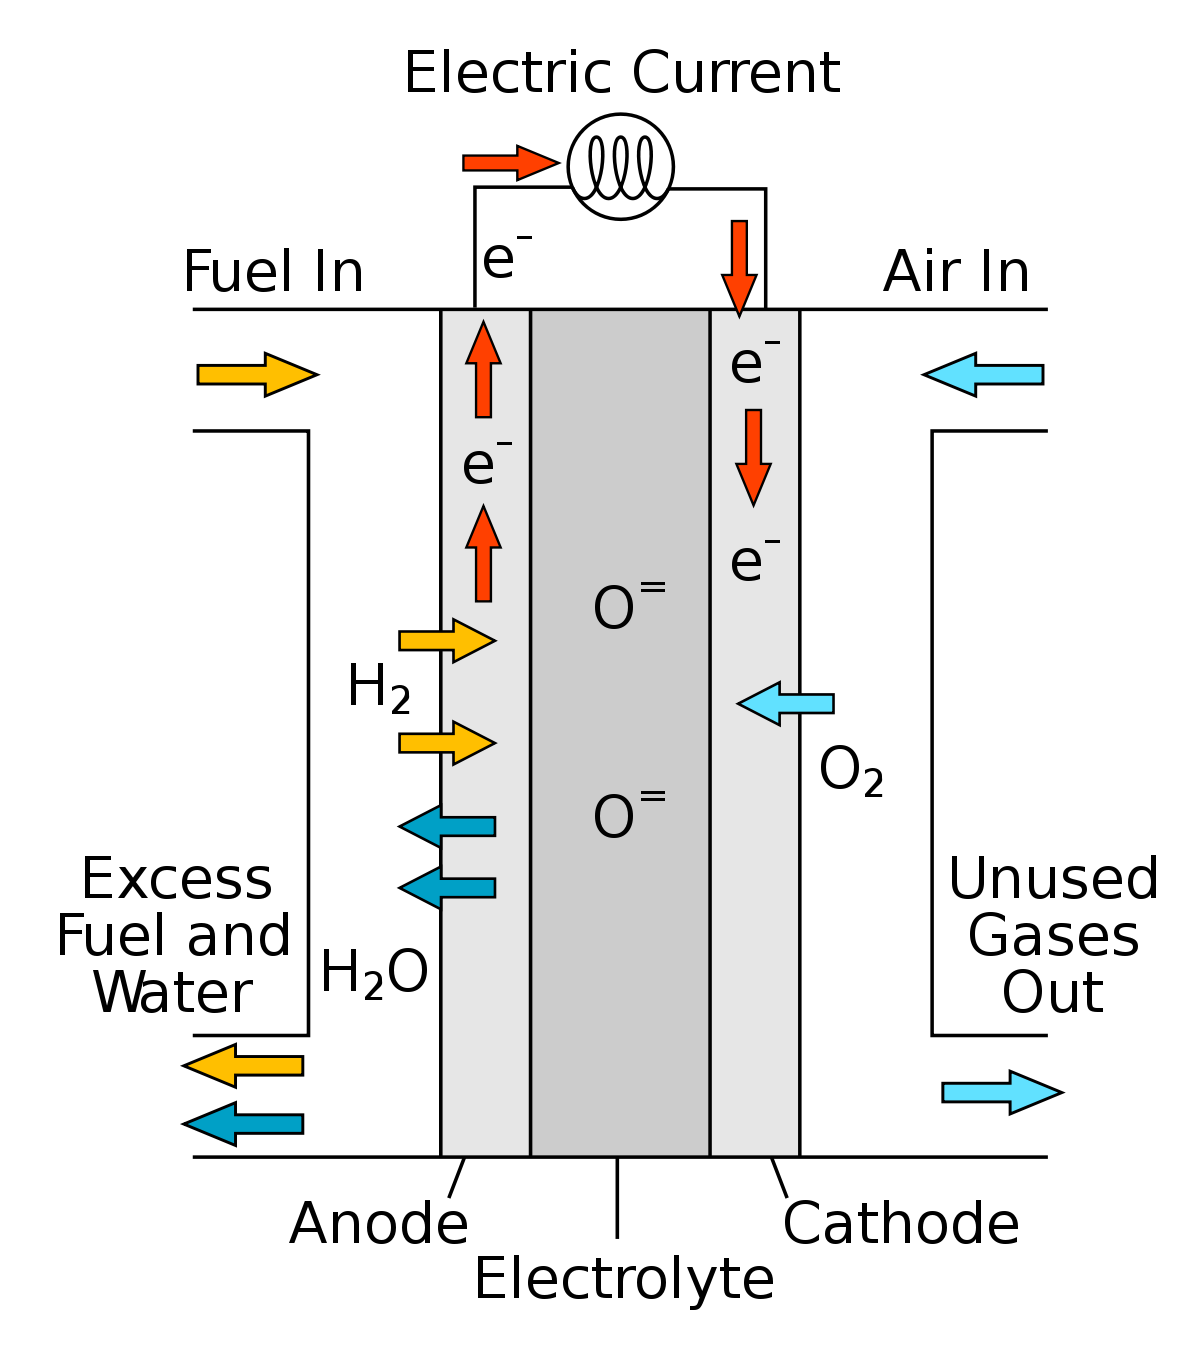
\includegraphics[scale=0.2]{1200px-Solid_oxide_fuel_cell.png}
        \caption{Simple diagram of SOFC-O operation \cite{lewisref1}}
        \label{fig:SOFCbasic}
    \end{figure}
    
    There are two main types of SOFCs, the differencing being which ions are conducted by the electrolyte. SOFC-Os have oxygen conducting electrolytes, whereas SOFC-Hs have hydrogen conducting electrolytes. Both variations will be considered in the model.
The fuel cell is composed of an electrolyte, either side of which is an anode and a cathode – one of which is significantly thicker than the others in order to give structural stability[2]. The fuel flow comes into contact with the anode, and the air flow with the cathode, where they are broken down by the high temperatures into hydrogen and oxygen ions, which are absorbed through the electrodes and react at the electrode/electrolyte interface, known as the ‘triple-phase boundary’, or TPB (anode interface for SOFC-O, cathode interface for SOFC-H). These ions react to form water, and the movement of electrons creates a current. This current flows along the fuel cells, separated by a conducting interconnect, and is the primary power output of the SOFC system.

  %  hello
  %        \subsubsubsection{wefawefawef}\label{lab
    \subsubsection{Cell Construction}
    
     \begin{figure}[h!]
        \centering
        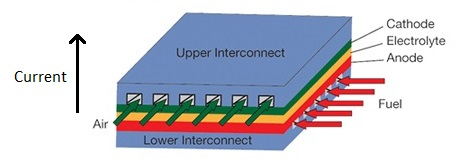
\includegraphics[scale = 4]{fuelcelldiagramedit.jpg}
        \caption{Diagram of a single fuel cell, that would be repeated in a vertical stack (adapted from \cite{lewisref8}}
        \label{fig:SOFCconstruction}
    \end{figure}
    
    The cell components must be made of materials with a similar coefficient of thermal expansion in order to prevent cracking when the fuel cell is heated up to operating temperature[]. The most common choice of electrolyte in literature is yttria-stabilised zirconia (YSZ) – an oxygen conducting electrolyte – chosen for it’s high ionic conductivity, and mechanical and thermal stability at high temperatures[]. It is also a very cost effective and sustainable choice, as it is found abundantly in the earth’s crust[]. The anode also needs to be a good conductor, and ideally should catalyse the breakdown of ammonia to increase fuel utilisation. Nickel mixed with YSZ is a good choice, allowing for similar thermal properties as the electrode, but also acting as a catalyst for the breakdown of ammonia[]. Using a nickel based anode means ammonia breakdown can be assumed to be 100\% at the anode surface[]. Similarly, the cathode is typically made of YSZ mixed with Sr-doped Lanthanum Manganite (LSM), as LSM catalyses the decomposition of oxygen into ions[]. These same materials were used in Ishak et al.’s model[5], which formed the basis for the model designed in this project. Not mentioned in Ishak’s paper was the interconnect, which must conduct electricity well at the operating temperature while also providing structural support to the fuel cell stack.  Typically, LaCrO3 ceramics are used[]. Fuel cells can either be planar or tubular in design, with literature suggesting that planar fuel cells have a greater power density, and are easier to manufacture, leading to a more efficient design[2].
    \subsubsection{Cell Potential}
    
\begin{figure}[htb]
    \centering
    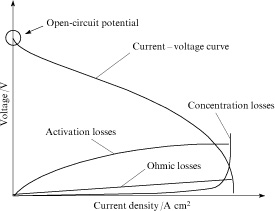
\includegraphics{voltagecurve.jpg}
    \caption{Typical voltage-current curve for a SOFC, showing the main potential losses \cite{lewisref9}}
    \label{fig:SOFCvoltagecurve}
\end{figure}
    
    Fuel cell performance is typically calculated using a graph of cell potential against current density, from which a curve for power density can be plotted, and the point of maximum power density can be observed. .Figure 3 demonstrates a typical voltage-current density plot for a SOFC. The shape is characterised by the three main potential losses – activation losses, ohmic (or resistive) losses, and concentration losses. Activation losses are the result of the activation energy of the electrodes, required to start the reactions at both[]. Ohmic losses are due to the resistive losses in the electrolyte as the electrons pass through it – the losses in the electrodes and the interconnects are considered negligible[]. The concentration losses are due to the changing concentration gradients between the electrode surface and the TPB. The reaction is rate-limited by the rate at which ions are absorbed in the electrodes, so the concentration losses sharply increase at high current densities, where more reactants are present at the TPB, and the concentration gradient rapidly drops and no ions move across the electrodes.[]
 The cell potential is calculated as the maximum theoretical voltage (the ‘Nersnt Voltage’) minus the losses across the electrodes and electrolyte[5]:
\begin{equation}
    V=E- \phi_{act,a} - \phi_{act,c}-  \phi_{\Omega}- \phi_{conc,a} -  \phi_{conc,c}			
\end{equation}
Where the Nernst voltage ‘E’ is found from the Nernst equation[2]:
\begin{equation}
E= E^0+  \Big (\frac{RT}{zF} \Big )  \frac{P_{H2} \sqrt{P_{O2} }}{P_{H2O} }				
\end{equation}
Where:				
\begin{equation}
E^0=  \frac{-\Delta G}{zF} =  \frac{(\Delta H^0-T \Delta S^0)}{zF} 						
\end{equation}
‘z’ is the number of electrons exchanged in the reaction, ‘F’ is Faraday’s constant, ‘ΔG’ is the Gibbs free energy, and ‘P’ is the partial pressure of the substance in subscript, at the electrode surface. 
$\phi_{act,a}$ and $\phi_(act,c)$ represent the losses due to ‘activation overpotential’ of the anode and cathode, respectively. These can be derived from the Butler-Volmer expression[3], giving:
\begin{equation}
\phi_{act,\gamma}=  \frac{RT}{F}   \sinh^{-1} \Big (⁡\frac{J}{zJ_{0,\gamma}} \Big )
\end{equation}
Where $\gamma$ represents the anode or cathode, and $J_{0}$ represents the exchange current density of the electrode. $J_{0,\gamma}$ is given in literature as[4]:

\begin{equation}
J_{0,a}= \gamma_{a} \Big (\frac{P_{H2}}{P^{0}}\Big ) \Big (\frac{P_{H2O}}{P^{0}} \Big )^{m} e^{ (\frac{-E_{act,a}}{RT}  )}			
\end{equation}

\begin{equation}
J_{0,c}= \gamma_{c} \Big (\frac{P_{O2}}{P^{0}} \Big )^{0.25} e^{(\frac{-E_{act,c}}{RT})} 					
\end{equation}
Where $E_{act}$ is the activation energy of the electrode, $P^0$ is the ambient pressure, and $\gamma_a$, $\gamma_c$ and $m$ are experimentally determined constants.
$φ_Ω$ represents the resistive losses in the electrolyte, and is calculated using:
\begin{equation}
\phi_{\Omega}=J\delta_{e} R_{\Omega} 						
\end{equation}
Where $J$ is the current of the cell, $\delta_e$ is the thickness of the electrolyte, and $R_\Omega$ is the resistivity of the electrolyte.
$\phi_{conc,a}$ and $\phi_{conc,c}$ represent the losses due to ‘concentration overpotential’. These are derived using the Dusty-Gas Model and are given in literature[5]. The equations differ depending on the type of electrolyte used in the cell:

SOFC-O:	
\begin{equation}
\phi_{conc,a} = \frac{RT}{2F} \ln \Big (\frac{P_{H2}^{TPB} P_{H2O}}{P_{H2} P_{H2O}^{TPB}} \Big )
\end{equation}

\begin{equation}
\phi_{conc,c} = \frac{RT}{4F} \ln \Big (\frac{P_{O2}}{P_{O2}^{TPB}} \Big ) 					
\end{equation}

SOFC-H:	
\begin{equation}
\phi_{conc,a}=  \frac{RT}{2F} \ln \Big (\frac{ P_H2 }{ P_H2^TPB } \Big )						
\end{equation}

\begin{equation}
\phi_{conc,c}=  \frac{RT}{2F} \ln \Big ( \frac{P_{H2O}^TPB \sqrt{{P_O2}}}{P_H2O \sqrt{P_O2^TPB}} \Big) 
\end{equation}

Where $P^{TPB}$ is the pressure of the substance in subscript, at the triple-phase boundary, which is the point at which the reaction takes place. These pressures are derived using an extended form of the Stefan-Maxwell model[6] (re-written according to the nomenclature of this report):

\begin{equation}
\frac{dy_{i}}{dx}=  \frac{-N_i}{D_{i,k}^{eff}}  - \frac{(y_j N_i- y_i N_j)}{D_{i,j}}					
\end{equation}
Where y is the mole fraction of the subscript gas (directly proportional to the partial pressure), N is the molar flux, $D_{i,j}$ is the diffusion coefficient, and $D_{i,k}^{eff}$ is the effective Knudsen coefficient. 
The current of the cell can be calculated by[2]:
\begin{equation}
J= \dot n zF					
\end{equation}
Where $n$ ̇ is the molar flow rate of hydrogen into the fuel cell. This is related to the molar flow rate of ammonia by the molar ratios of the chemical equations.

    \subsubsection{Cell Reaction}
    The reaction for ammonia decomposition is:
    \begin{equation}
\frac{2}{3} 〖NH〗_3  →  H_2+  \frac{1}{3} N_2					
\end{equation}
The reaction inside the fuel cell is:
\begin{equation}
H_2+  \frac{1}{2} O_2  → (x)H_2 O+(1-x)H_2+  \frac{1}{2} O_2
\end{equation}
Where x is the fraction of hydrogen that is utilised in the reaction. All terms in Equations 14 and 15 are in the gaseous state. From these we can see that the molar ratios of substances, and calculate the mole fractions of the substances at the electrodes before the reaction takes place. We can also calculate that the molar air to fuel ratio must be 3.57, and therefore is 3.57 by volume, by the ideal gas assumption. This assumption is valid given the extremely high temperatures of the gases.[]

\subsection{Design Procedure}
    \subsubsection{Model Design}
    A model was designed using MATLAB in order to simulate the effect of changing the various design parameters on the cell’s power density. The various properties of the gases involved in the reaction, and the material properties of the electrodes and electrolyte, were used as inputs, and the various design equations implemented to calculate the final cell potential. The Extended-Stefan-Maxwell equations formed two separate systems of ordinary differential equations, which were solved using the MATLAB function ‘ode45’. Plotting the cell potential, and cell power density, against the current density allowed the maximum power output to be found graphically, and therefore the optimal operating conditions could be found.
    \subsubsection{Experimentation}
    By changing the operating conditions and material properties in the model, different conditions could be tested so that the optimal cell design could be found. Due to a limited variety of appropriate materials in literature, there were very few different parameters that could actually be changed, and therefore investigated – as such a comparison between SOFC-O and SOFC-H was not possible. The most important of these were the operating temperature and pressure, and the thickness of the electrodes and electrolyte in the cell. A ‘control’ configuration was decided on, so that results could be compared, and then each variable was changed to see the effect on the maximum power density.
The control configuration was heavily based on the design used by Ishak et al.[5], using nickel mixed with YSZ (yttria-stabilized zirconium) for the anode, a YSZ electrolyte, and a LSM-YSZ cathode. Though the final design would require one component to be significantly larger than the other to give structural stability, they were all equally thick at 50 micrometres. This was so that the effect of changing the component thicknesses could be clearly demonstrated. The operating conditions were a temperature of 1073K, and atmospheric pressure. For all tests, the ammonia decomposition was assumed to be 100\% (due to the Nickel present at the anode, which catalyses the breakdown), and the hydrogen utilisation assumed to be 80%[20].

    \subsubsection{Results}
    The effects on the performance by changing the operating conditions are as shown:
    
    GRAPH
    \begin{figure}[h!]
        \centering
        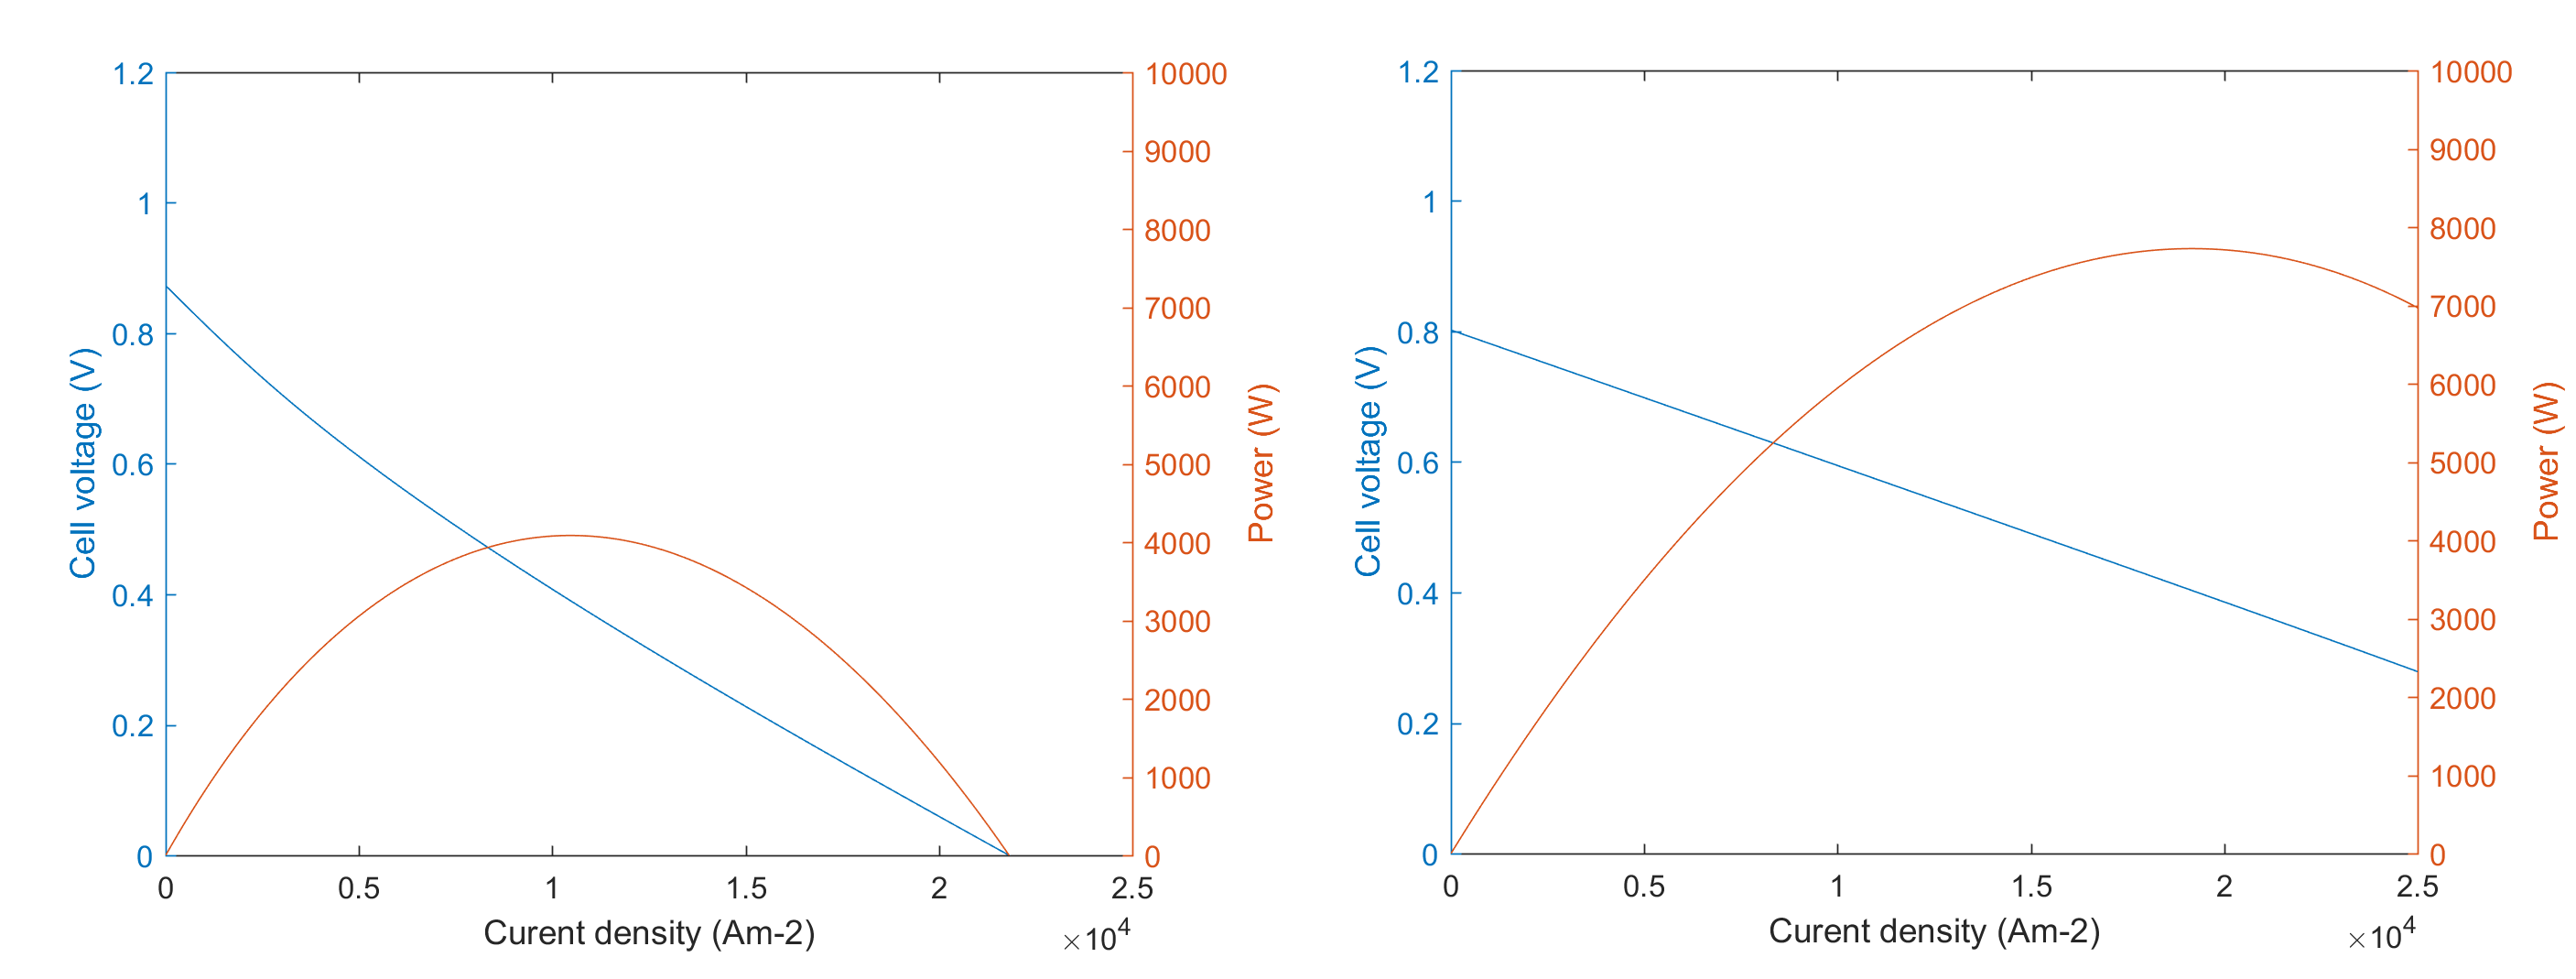
\includegraphics[width=1\textwidth]{controlvsinc_temp.png}
        \caption{Voltage and Power vs Current Density for the control configuration (left) and an increased temperature of 1273K (right)}
        \label{fig:SOFCtempinc}
    \end{figure}
    
      GRAPH
      \begin{figure}[h!]
        \centering
        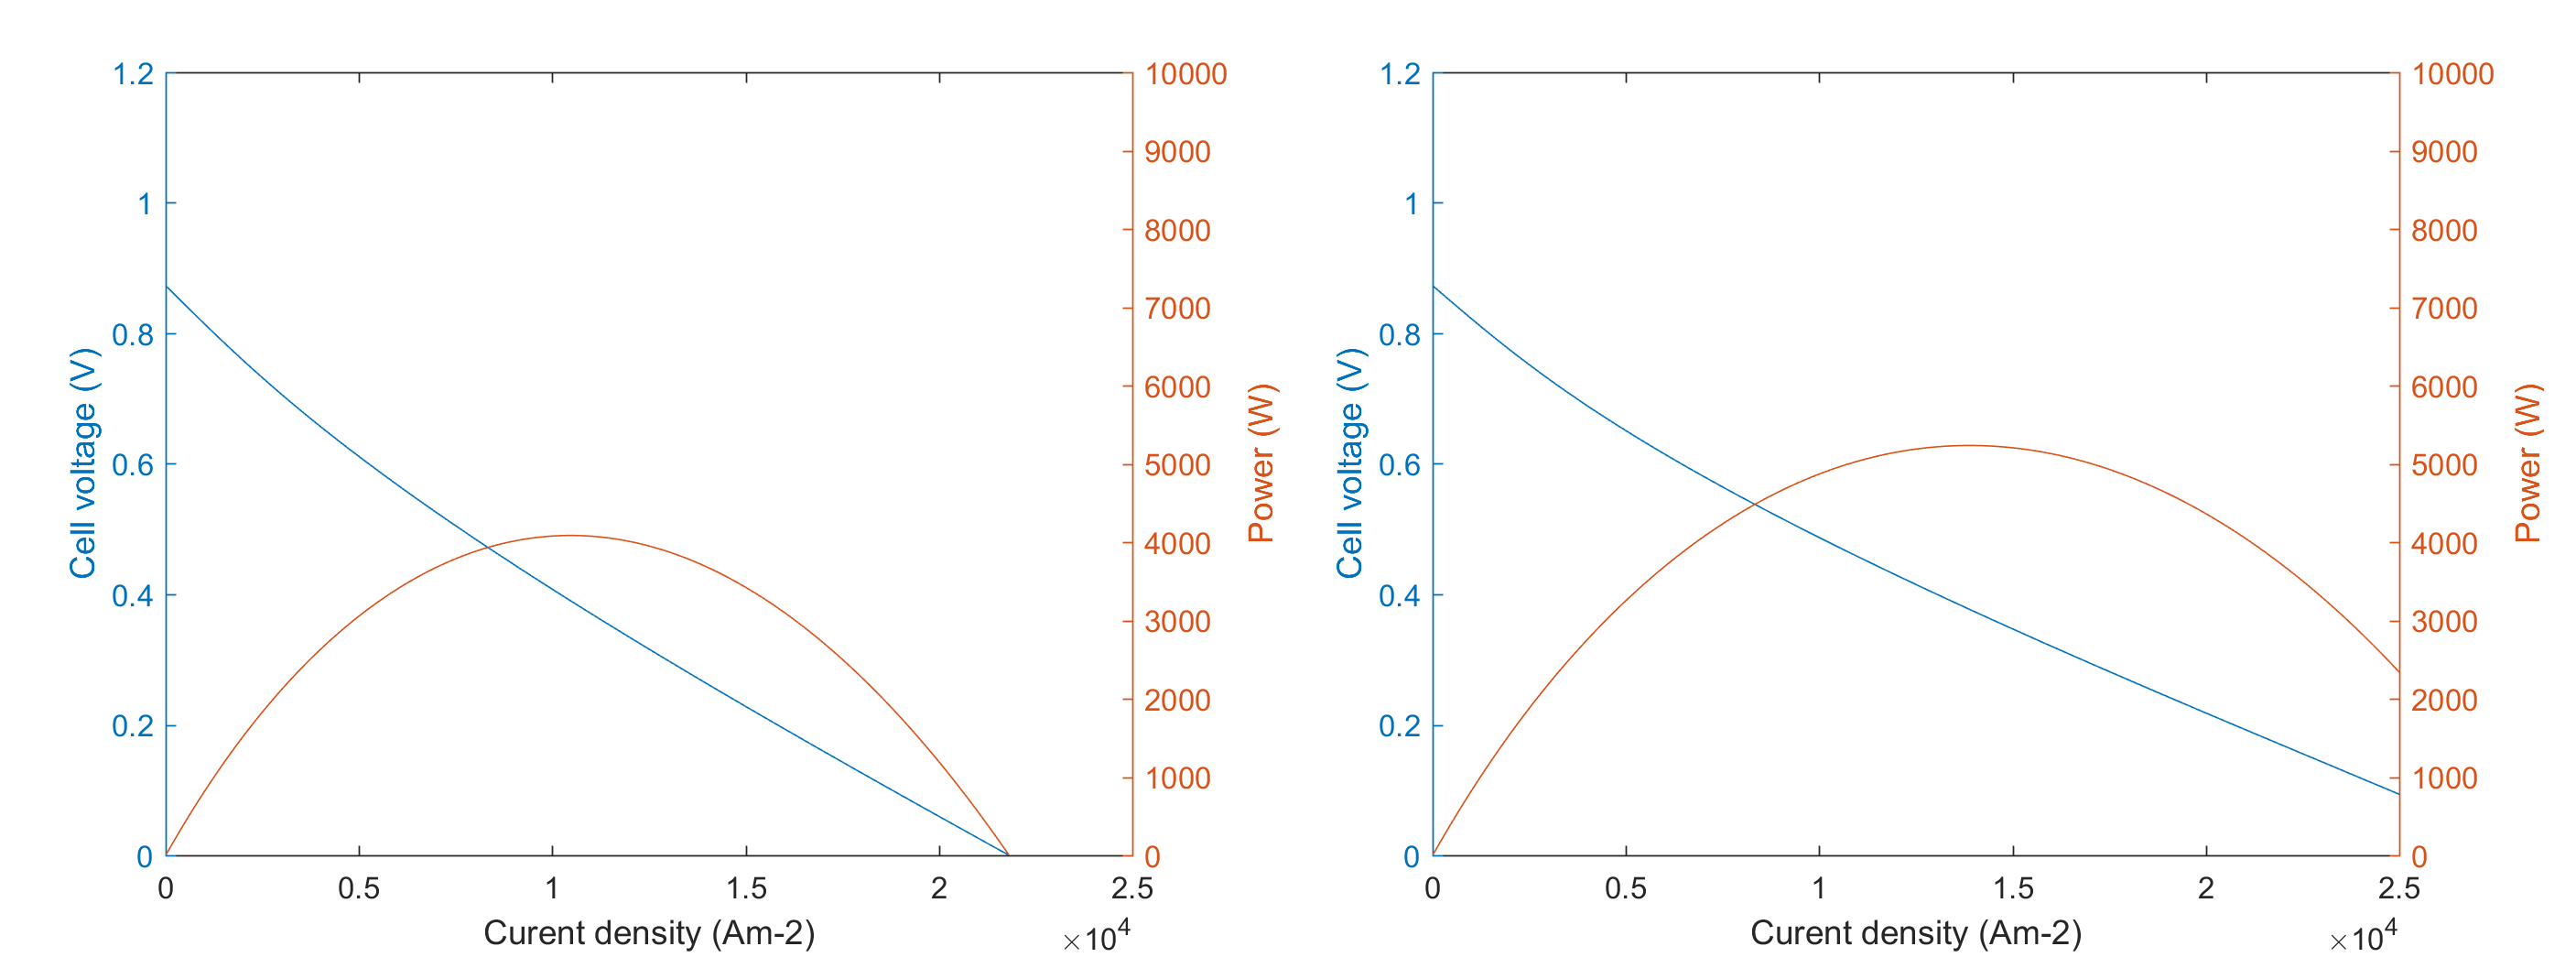
\includegraphics[width=1\textwidth]{controlvsinc_pres.png}
        \caption{Voltage and Power vs Current Density for the control configuration (left) and an increased pressure of 5 bar (right)}
        \label{fig:SOFCpresinc}
    \end{figure}
    
    Increasing temperature and pressure both increase the cell’s maximum power density, but increasing temperature has the most significant effect.
    The effect of changing the support method is as shown – dimensions in micrometres:

  GRAPH
  \begin{figure}[h!]
      \centering
      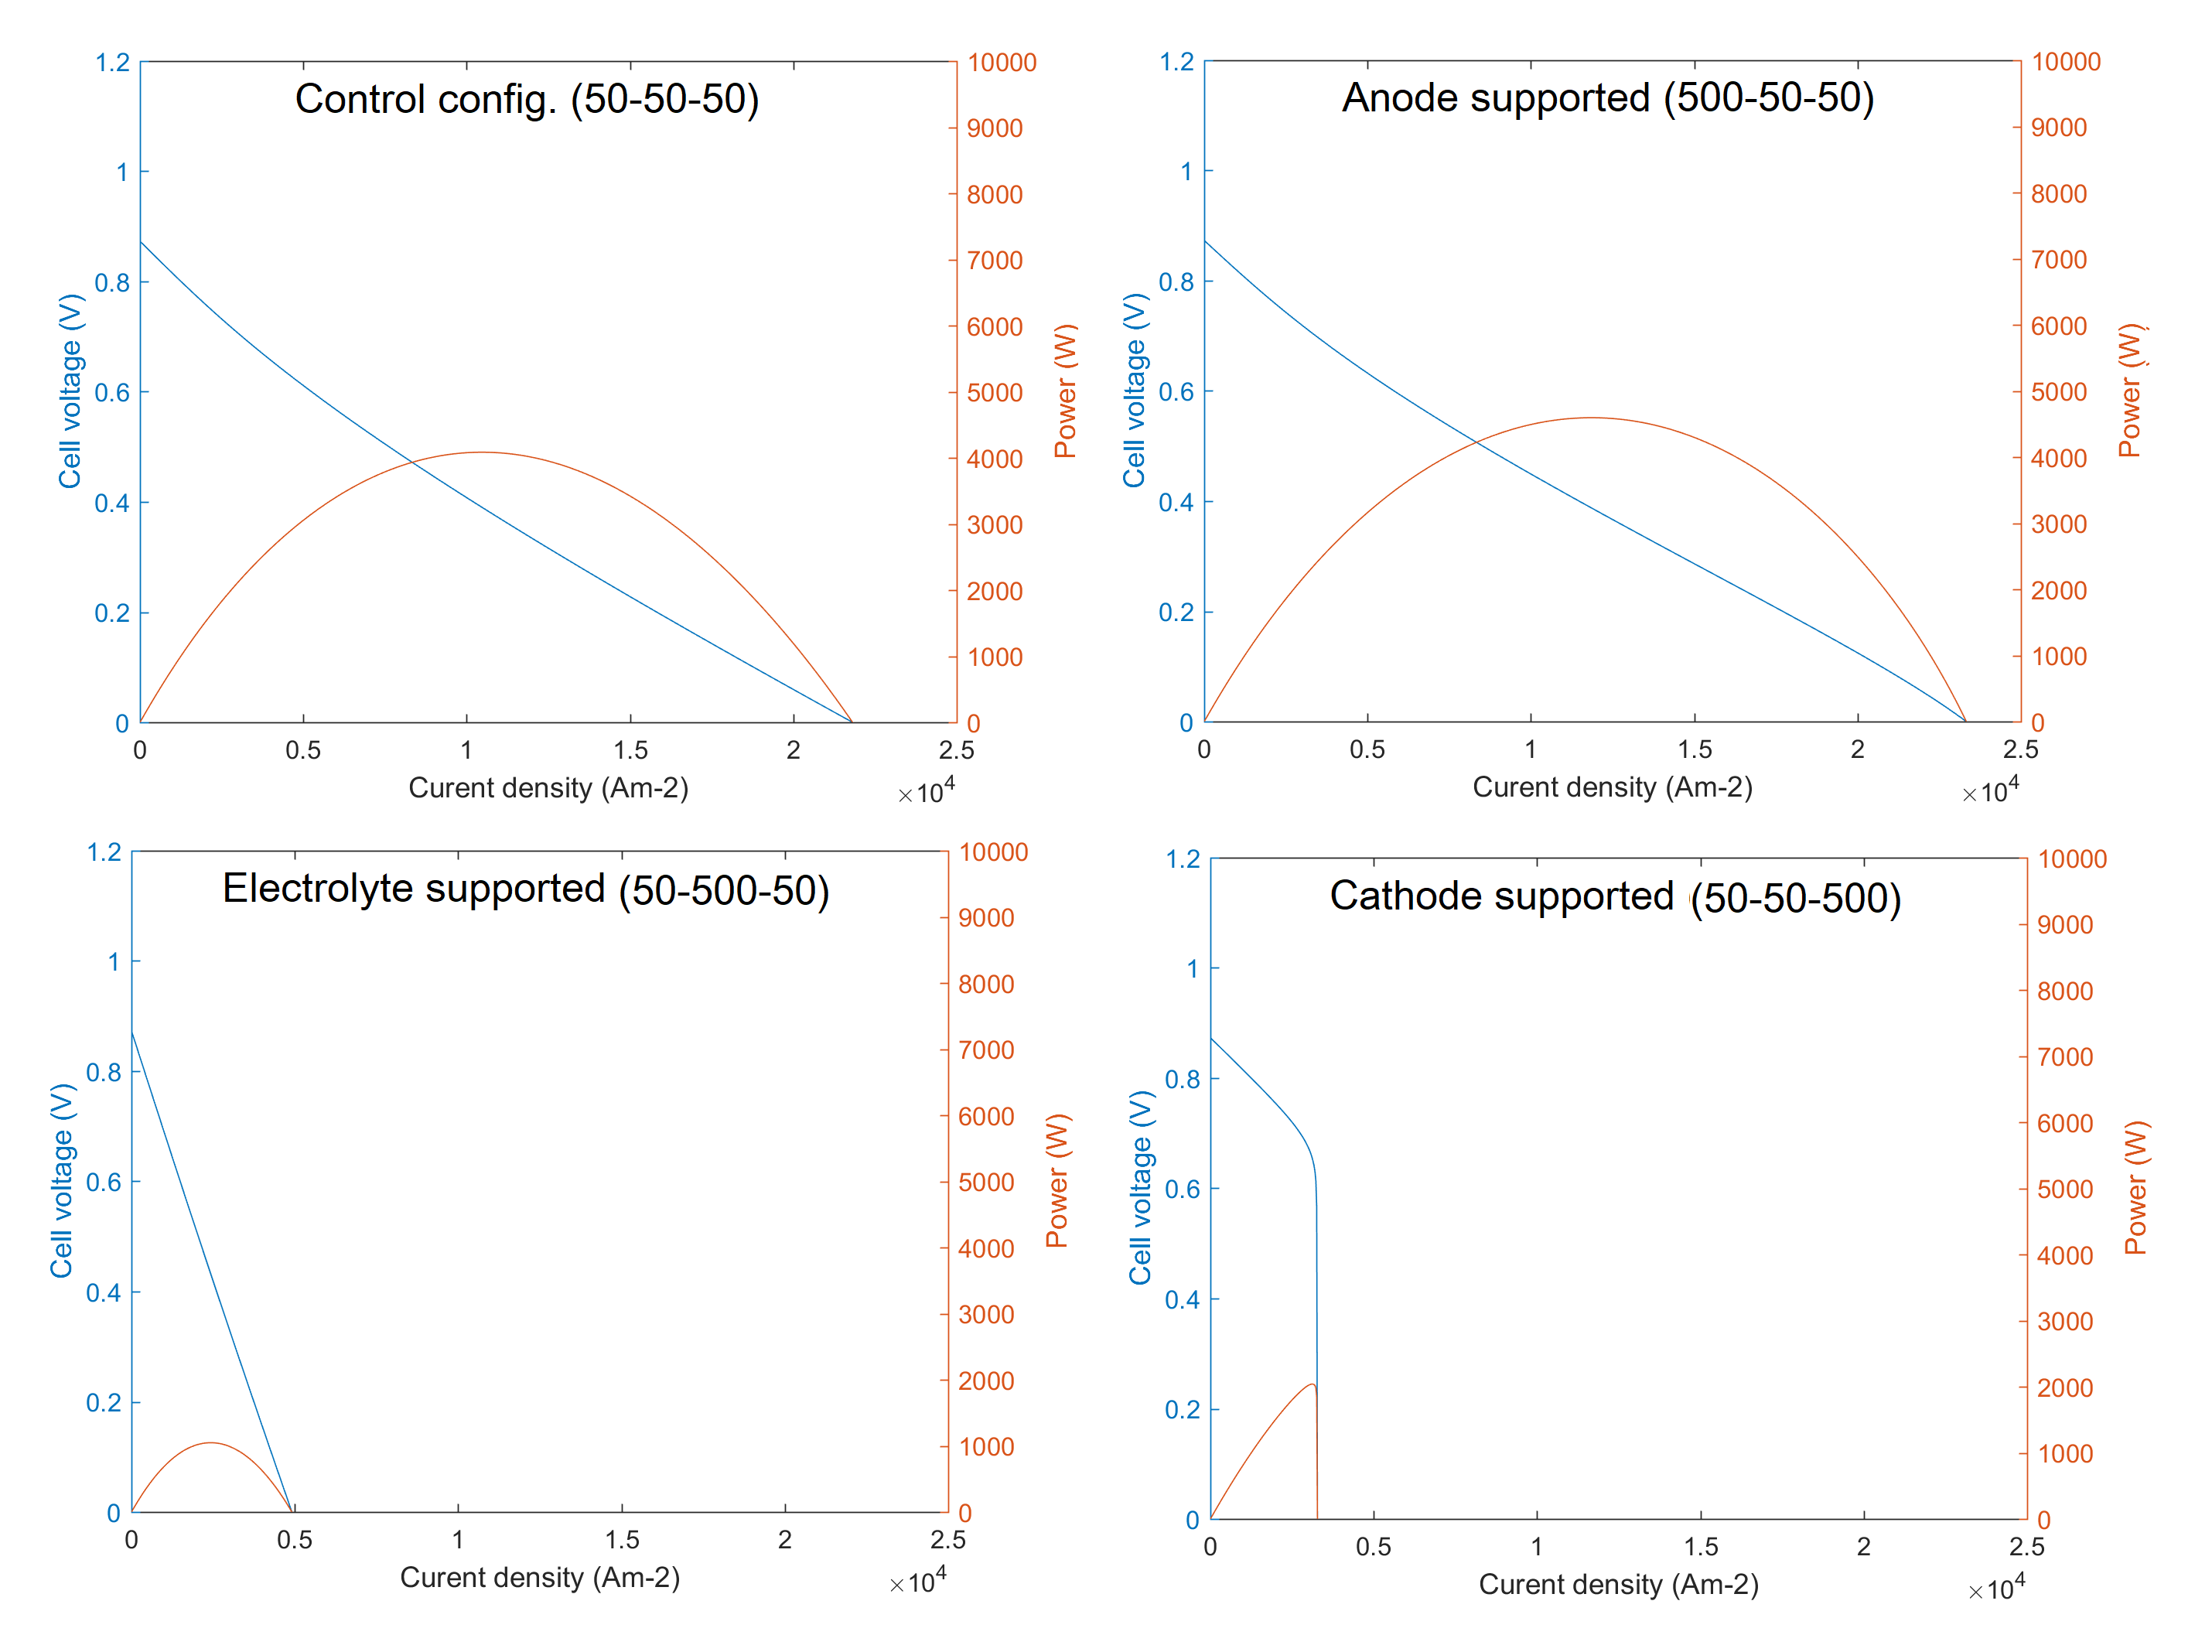
\includegraphics[scale=0.6]{support_comparison.png}
      \caption{Caption}
      \label{fig:SOFCsupport}
  \end{figure}
  
    It is clear from Figure 6 that an anode-supported cell has superior power density. The increased anode thickness causes the power density to increase, whereas the electrolyte and cathode supported cells result in significant decreases in power density. The electrolyte supported case can be explained by the significant increase in ohmic losses. The cathode supported case is likely an exaggerated result due to the failure of the ESM model to account for the rate of change of concentration gradient, causing it to drop rapidly, resulting in the very sudden increase in concentration losses (evident by the shape of the graph). However, the conclusions drawn are supported by Adolfo’s thesis[2], and it is widely stated in literature that anode-supported cells are superior. 
    \
   \
   \
   \
   \
    \subsubsection{Final Cell Stack Design}
    Based on these conclusions, some further testing was performed and a final design was decided on:
Ni-YSZ/YSZ/LSM-YSZ (500-20-30), at 1273K and atmospheric pressure

GRAPH
\begin{figure}[h!]
    \centering
    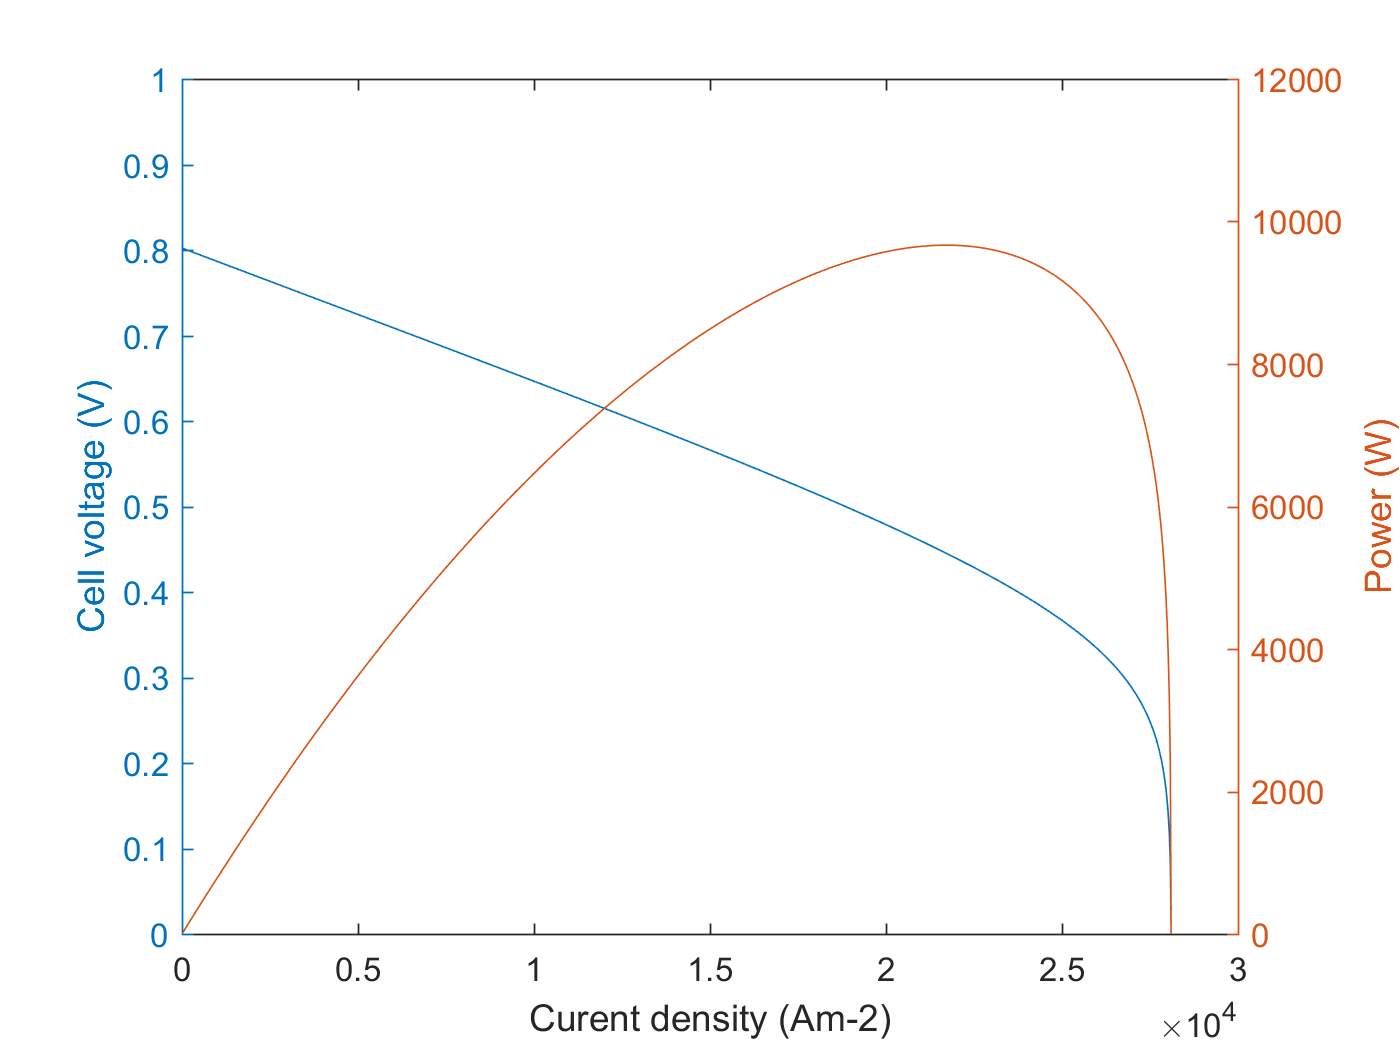
\includegraphics[scale = 0.25]{power_voltage_against_current.png}
    \caption{Caption}
    \label{fig:SOFCfinal}
\end{figure}

By choosing a cell area of 0.3m x 0.3m, currently the largest that can be produced[10], the power produced per fuel cell can be shown to be 870W. To fulfil the demand of 230MW, the cells themselves will need to produce 150MW, as the integrated turbine will produce the remaining 80MW. Therefore, just under 172,500 cells will be required. Stacks of 1150 cells will be used, each producing just slightly over 1MW, requiring 150 stacks in total.
        
\subsection{Integrated Gas Turbine}
    \subsubsection{Thermodynamic Analysis}
        The reaction in the cell is exothermic overall. Ammonia decomposition absorbs 37.278kJ per mole of H2 and the cell reaction produces 199.578kJ per mole of H2, so 162.3kJ per mole of H2 is produced overall – or 243.45kJ per mole of NH3. This heat can be used to heat up the inlet gases to the operating temperature. Therefore, the inlet temperature of the fuel and air can be calculated using the equation:
\begin{equation}
Q_{heat}- Q_{loss}=mc_{p(T_i} )  (T_{SOFC}-{ T_i)} 				
\end{equation}
Where $T_i$ is the temperature of the inlet reactants, in Kelvin. As the value of $c_p$ depends on the inlet temperature, it must be found iteratively. A short MATLAB script was devised for this purpose. $Q_{heat}$ could be calculated as the total energy produced by the reaction in the SOFC system, subtracting the energy released as electricity.
 $Q_{loss}$ represents the heat loss from the SOFC system. This was found by calculating the one-dimensional overall heat transfer coefficient (HTC) between the fuel cell and its surroundings, and applying it to the total area of the stack.
 \begin{equation}
 Q_{loss}=UA(T_{SOFC}- T_{amb})					
 \end{equation}
Where U is the overall HTC, A is the total area of the SOFC stack, and $(T_{SOFC}- T_{amb})$ is the difference between the SOFC temperature and the ambient temperature.


DIAGRAM


To simplify this calculation, it is assumed that the fuel cell stacks have a uniform temperature of 1273K. This assumption is acceptable provided the Biot number is less than 0.1. This can be calculated by:
\begin{equation}
 B_i=h_{conv} \Sigma_{i}^{n} \frac{t_i}{k_i}  						
 \end{equation}
Where $h_{conv}$ is the convective HTC of the overall body, $t_i$ is the thickness and $k_i$ is the thermal conductivity of component $i$. As the materials of the anode, cathode, and electrolyte are all variations of YSZ, we can assume the value of $k_i$ to be the same for each. The values are given in Table \ref{tbl:HTCcoeff}.

\begin{table}[h!]
\centering
\caption{Table of component HTC's and thicknesses \cite{lewisref11} \cite{lewisref12}}
\label{tbl:HTCcoeff}
\begin{tabular}{|c|c|c|}
\hline
\textbf{Component}         & \textbf{Conductive HTC ($\text{Wm}^{-1}\text{K}^{-1}$)} & \textbf{Thickness (m)}     \\ \hline
Interconnect               & 1.9                               & 1*10^{-3}   \\ \hline
Electrodes and Electrolyte & 2.5                               & 600*10^{-6} \\ \hline
\end{tabular}
\end{table}

And $h$ is given as 16 Wm-2K-1[7]. The Biot number is calculated as 0.012– therefore the assumption is valid. Due to the very high temperature of the system, heat loss from radiation is the most significant. The radiative heat transfer coefficient can be calculated using the equation[13]:
\begin{equation}
h_{rad}= \epsilon \sigma (T_{SOFC}^2 + T_{amb}^2)(T_{SOFC}+ T_{amb}) 			(17)
 \end{equation}
Where $\epsilon$ is the emissivity of the body, and $\sigma$ is the Stefan-Boltzmann constant. Assuming an emissivity value of 0.8[7], the coefficient is calculated as 121.8 Wm-2K-1. The conductive and convective heat transfer coefficients are also accounted for. The convective HTC is 16Wm-2K-1 as given previously, and the conductive heat transfer is given by:
\begin{equation}
 h_{cond}=\frac{k}{t}						
  \end{equation}
Where k and t are the thermal conductivity and thickness of the insulation around the SOFC. The overall HTC can then be calculated by:
\begin{equation}
 U=  \frac{1}{\frac{1}{h_{rad}} + \frac{1}{h_{conv}} + \frac{1}{h_{cond}} }						
   \end{equation}
The heat loss from the stack can be reduced significantly depending on the thickness of insulation, and the material used. The only insulator suitable for the high temperature of the SOFC stack is mineral wool[15], with a typical thermal conductivity of 0.04Wm-1K-1[14]. Heat loss against insulation thickness is plotted in Figure 8:

GRAPH
\begin{figure}
    \centering
    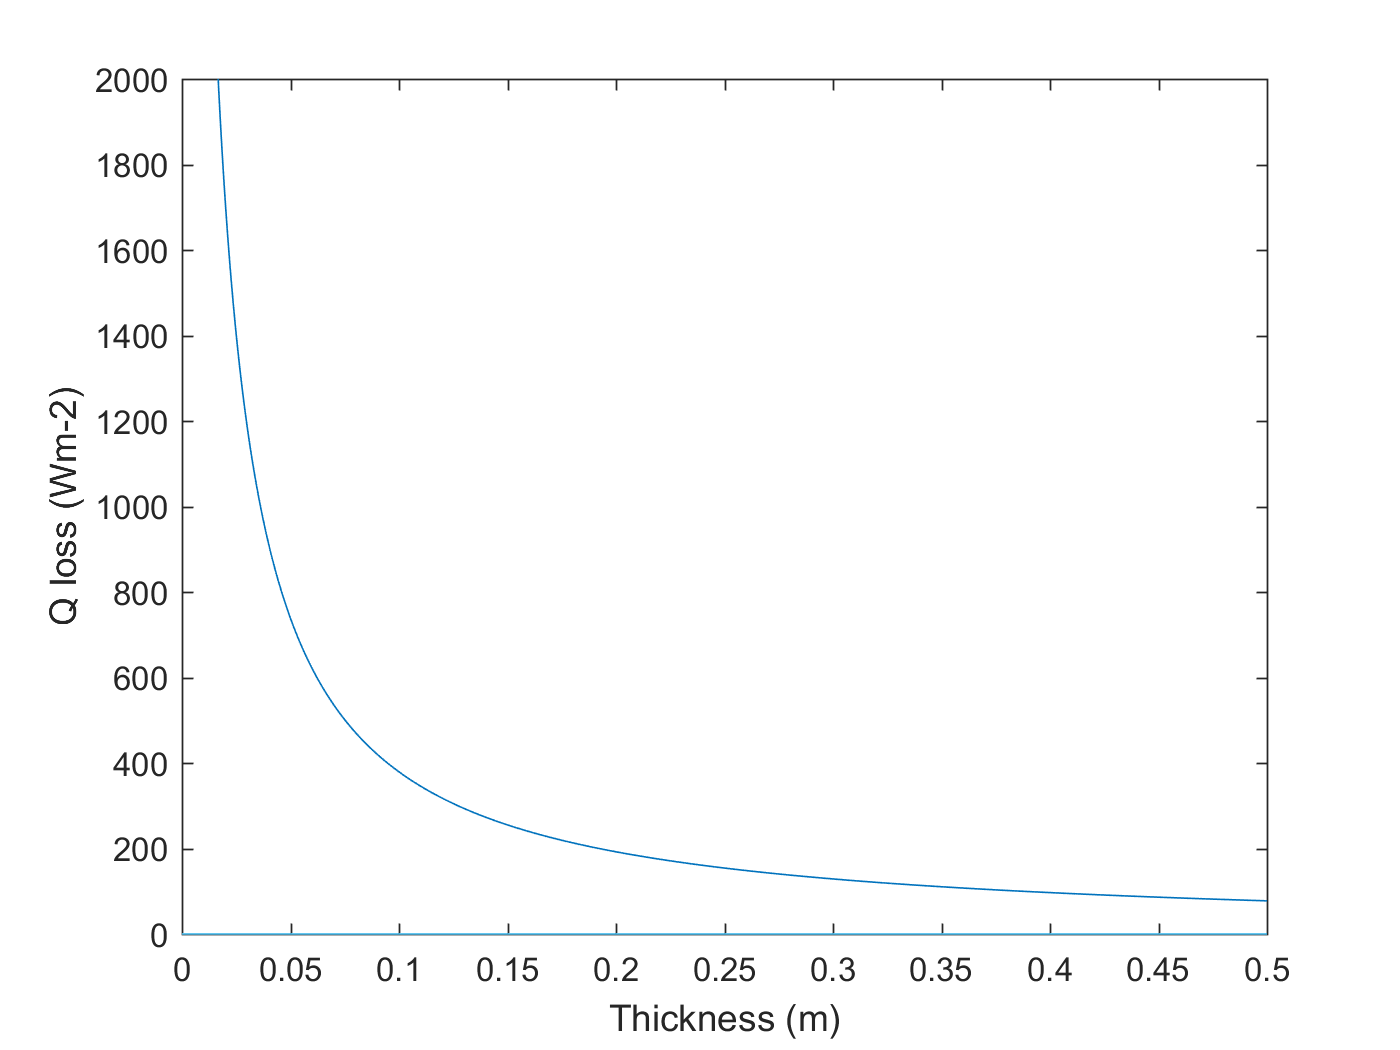
\includegraphics[scale=0.25]{insulation_thickness.png}
    \caption{Caption}
    \label{fig:my_label}
\end{figure}

It can be seen that diminishing returns occur almost immediately after a thickness of 0.05m. As such, using this value, the total heat loss per cell is calculated using Equation 15, giving a heat loss per cell value of 1.488W, which for the entire system is 256.68kW. Using Equation 14 iteratively, recalculating the $c_{p}(T_i )$  value for the inlet gases each time, the required inlet temperature for the fuel and air is 600K.
    \subsubsection{Secondary Gas Turbine Cycle}
        5.2 Secondary Gas Turbine Cycle
Knowing that the inlet temperature for the reactant streams is 600K, the hot exhaust from the fuel cells can be used to heat the streams to this desired temperature. The fuel is stored at as a liquid at 243K and ambient pressure, so must first be heated slightly to convert it to the gaseous state. The gas can then be directed through a heat exchanger operating counter currently to the exhaust stream, where it is heated to 600K. The exhaust flow can also be used to heat up the air flow, from ambient temperature to 600K. The heat exchange can be calculated using:
\begin{equation}
 〖(mc_p \Delta T)〗_{\text{exhaust stream}}= 〖(mc_p \Delta T)〗_{\text{inlet stream}}			
 \end{equation}
$c_p$ for the fuel and air streams can be taken from the JANAF tables, and can be calculated for the exhaust stream at different temperatures by:
\begin{equation}
 c_p= \Sigma_{i}^{n}〖c_{p_{i}}  y_i						
  \end{equation}
Where $y$ is the mole fraction of the component $i$ in the exhaust mixture. 


TABLE
\begin{table}[h!]
\centering
\caption{My caption}
\label{lewisHEXtemps}
\begin{tabular}{|c|c|c|c|c|}
\hline
\textbf{Heat Exchanger} & \textbf{Reactant inlet temp (K)} & \textbf{Reactant outlet temp (K)} & \textbf{Exhaust inlet temp (K)} & \textbf{Exhaust outlet temp(K)} \\ \hline
HEX 1 (Fuel Stream)     & 243                              & 600                               & 1273                            & 1205                            \\ \hline
HEX 2 (Air Stream)      & 298                              & 600                               & 1205                            & 1030                            \\ \hline
\end{tabular}
\end{table}

It can be seen in table 2 that the exhaust stream is still extremely hot, at 1030K. This heat is used to drive a secondary gas turbine cycle, which can be used to generate additional work and increase the overall efficiency of the system. By reducing the exhaust stream temperature to 298K, the exhaust stream can safely be ejected to the atmosphere.

DIAGRAM

Modelling the secondary gas turbine cycle as a Brayton cycle, the cycle can be analysed with the following equations:
\begin{equation}
T_{2,s}= T_1 \Big (\frac{P_2}{P_1} \Big )^{\frac{\gamma-1}{\gamma}}					
\end{equation}
\begin{equation}
T_2= T_1+  \frac{(T_{2,s}- T_1)}{\eta_c} 					
\end{equation}
\begin{equation}
T_{4,s}=\frac{T_3}{\Big (\frac{P_2}{P_1} \Big )^{\frac{\gamma-1}{\gamma}}} 						
\end{equation}
\begin{equation}
T_4= T_3- \eta_t (T_3- T_{4,s})				
\end{equation}
\begin{equation}
W_{in} \text{(compressor)}= c_p (T_1- T_2)(m_{air} ) ̇				
\end{equation}
\begin{equation}
W_{out} \text{(turbine)}= c_p (T_3- T_4)(m_{air} ) ̇				
\end{equation}
\begin{equation}
\text {Net power out}=W_{out} - W_{in}		
\end{equation}
Where $T_i$ is the temperature at point $i$, $P_i$ is the pressure at point $i$, $\gamma$ is the ratio of specific heats of air, $\eta_t$ and $\eta_c$ are the isentropic efficiencies of the turbine and compressor respectively, $c_p$ is the specific heat capacity, $W_{in}$ is the work done on the compressor, $W_{out}$ is the work done by the turbine, and $m_{air}$ is the mass flow rate of air through the cycle. $T_1$ and $P_1$ are the ambient conditions of atmospheric air, $\gamma$ for air is 1.4, and $\eta_t$ and $\eta_c$ are assumed to be 0.8[]. $T_3$ is calculated using Equation 20 across a third heat exchanger, using $T_2$ as the inlet air temperature. This depends on $P_2$, which is chosen to be 15 bar. This is because anything under 12 bar was found to cause the power output to decrease with increasing mass flow of air. $m_{air}$ is determined graphically so as to optimise the value of $T_3$, and subsequently optimise the net power produced by the cycle. This was done using MATLAB and produced the following results:


GRAPH
\begin{figure}[h!]
    \centering
    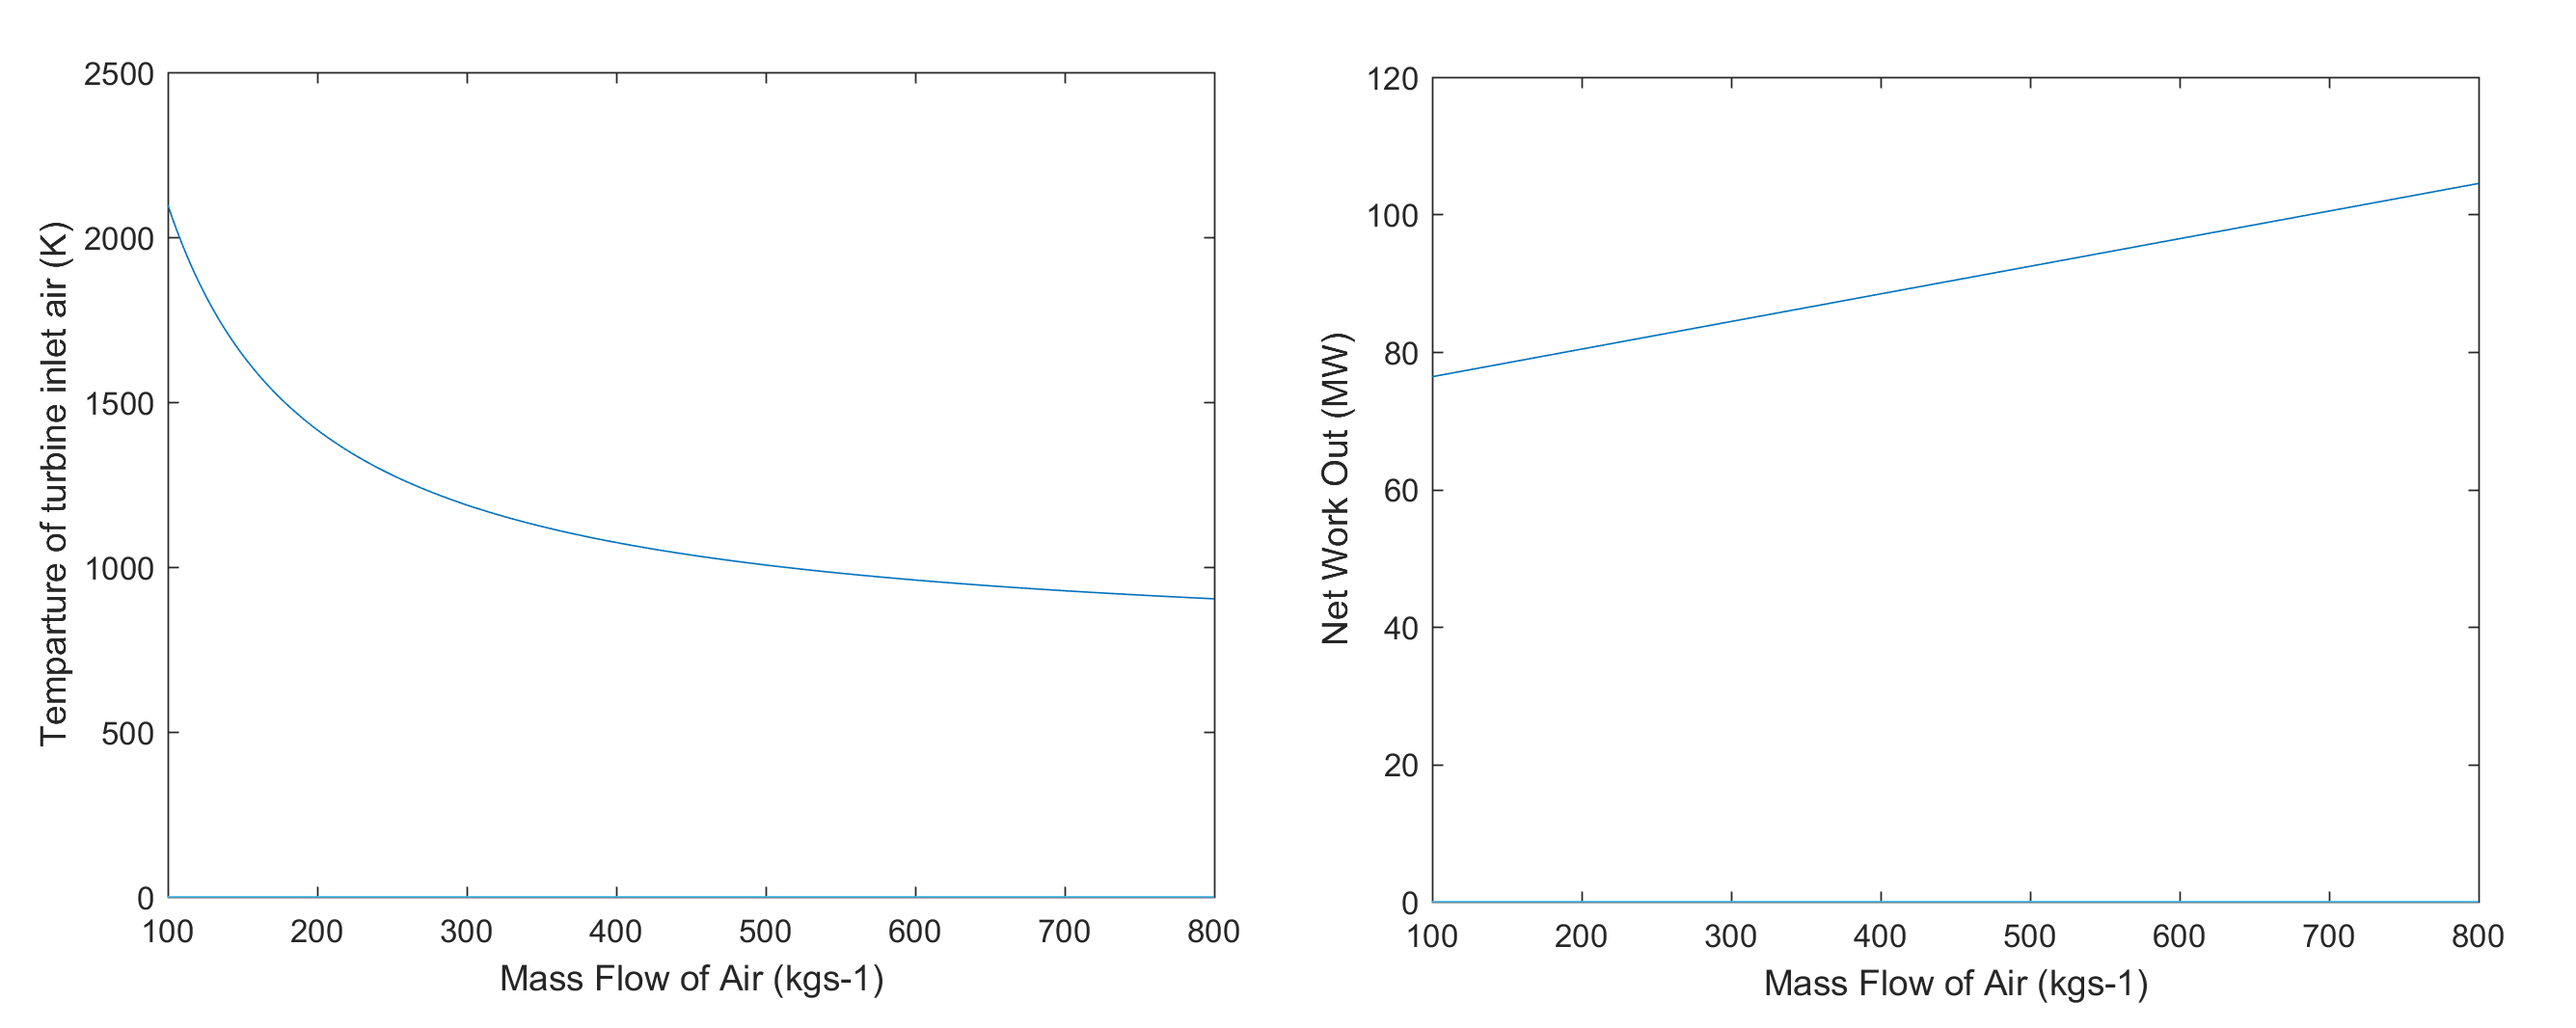
\includegraphics[scale=0.6]{t3_and_nw_vs_mass_flow_final.png}
    \caption{Caption}
    \label{fig:my_label}
\end{figure}

Flow rates below 100kgs-1 were ignored as the temperatures were unfeasibly high. The turbine inlet temperature was constrained by the melting point of the turbine itself. Using the melting point of stainless steel as a guideline, at 1783K[16], and erring on the side of caution, a mass flow rate of 200kgs-1 was taken, giving an inlet temperature of 1416K, and a net work value of 80MW. An advantage of this is that the power output can be increased simply by increasing the mass flow rate, if need be.
\\
DIAGRAM
\\

    \subsubsection{Heat Exchangers}
    
    Knowing the desired temperatures of the various streams, the heat exchangers can be analysed in more detail. In order to properly estimate the cost of the plant, the areas of the heat exchangers must be calculated. The general equation for heat exchanger design is:
\begin{equation}
Q=UA\Delta T_{LM}						
\end{equation}
Where $Q$ is the heat transferred, $U$ is the overall heat transfer coefficient, $A$ is the area, and $\Delta T_{LM}$ is the log mean temperature difference over the exchanger. Assuming the heat exchangers are ideal, with no losses, constant pressure and of the shell and tube design, the typical values of heat transfer coefficients for a variety of stream combinations can be found. As all the streams are gases, not including steam, the value of the HTC lies between 10 and 50 Wm-2K-1[18]. Taking a conservative average value of 25Wm-2K-1 for all streams, the heat exchanger analysis is as follows:

TABLE
\begin{table}[h!]
\centering
\caption{My caption}
\label{my-label}
\begin{tabular}{|c|c|c|c|c|}
\hline
\textbf{Heat Exchanger} & \textbf{Q (MW)} & \textbf{U (Wm-2K-1)} & \textbf{T log mean (K)} & \textbf{A (m2)} \\ \hline
HEX 1                   & 14.36           & 25                   & 809                     & 710             \\ \hline
HEX 2                   & 36.38           & 25                   & 666                     & 2185            \\ \hline
HEX 3                   & 146.11          & 25                   & 410                     & 14255           \\ \hline
\end{tabular}
\end{table}


\subsection{System Controller}
As stated in section 3.3, the desired air to fuel ratio (AFR) for molar equilibrium is 3.57. This ratio is desirable as it maximises the efficiency by allowing the reaction to take place, while minimising the amount of wasted air or fuel that doesn’t react. To achieve this, a controller was designed such that the AFR can be set by an operator, and any changes to the fuel flow will cause the air flow to change accordingly. The controller was designed using Simulink, and models the movement of valves that control the volume flow rate of fuel and air.
The transfer function for a typical valve was found to be[17]:
\begin{equation}
\frac{1}{\Big (\frac{1}{52s}+1 \Big )}						
\end{equation}
A valve ‘block’ was created in Simulink using this transfer function. Saturation was introduced, in order to accurately model the valves. The valves can only be fully open, fully closed, or somewhere in between, so the controller model needs to account for this. Similarly, non-idealities are introduced to make the model more realistic, adding in errors to account for things such as friction, or small pipe leakages. This formed the basis for the ‘plant’, representing the fuel valve, and a feedback loop was created using a PID controller, where the input is a step change in fuel flow. The PID controller was then tuned to give an appropriately smooth and quick response. This plant was duplicated for the air valve, but with the input being the fuel flow multiplied by the AFR to give the optimal air flow. The results of the simulation are shown in Figure X. The step change occurs at 0.2 seconds, and it is clear that a smooth response happens in under 0.1 seconds.

GRAPH
\begin{figure}[t!]
    \centering
    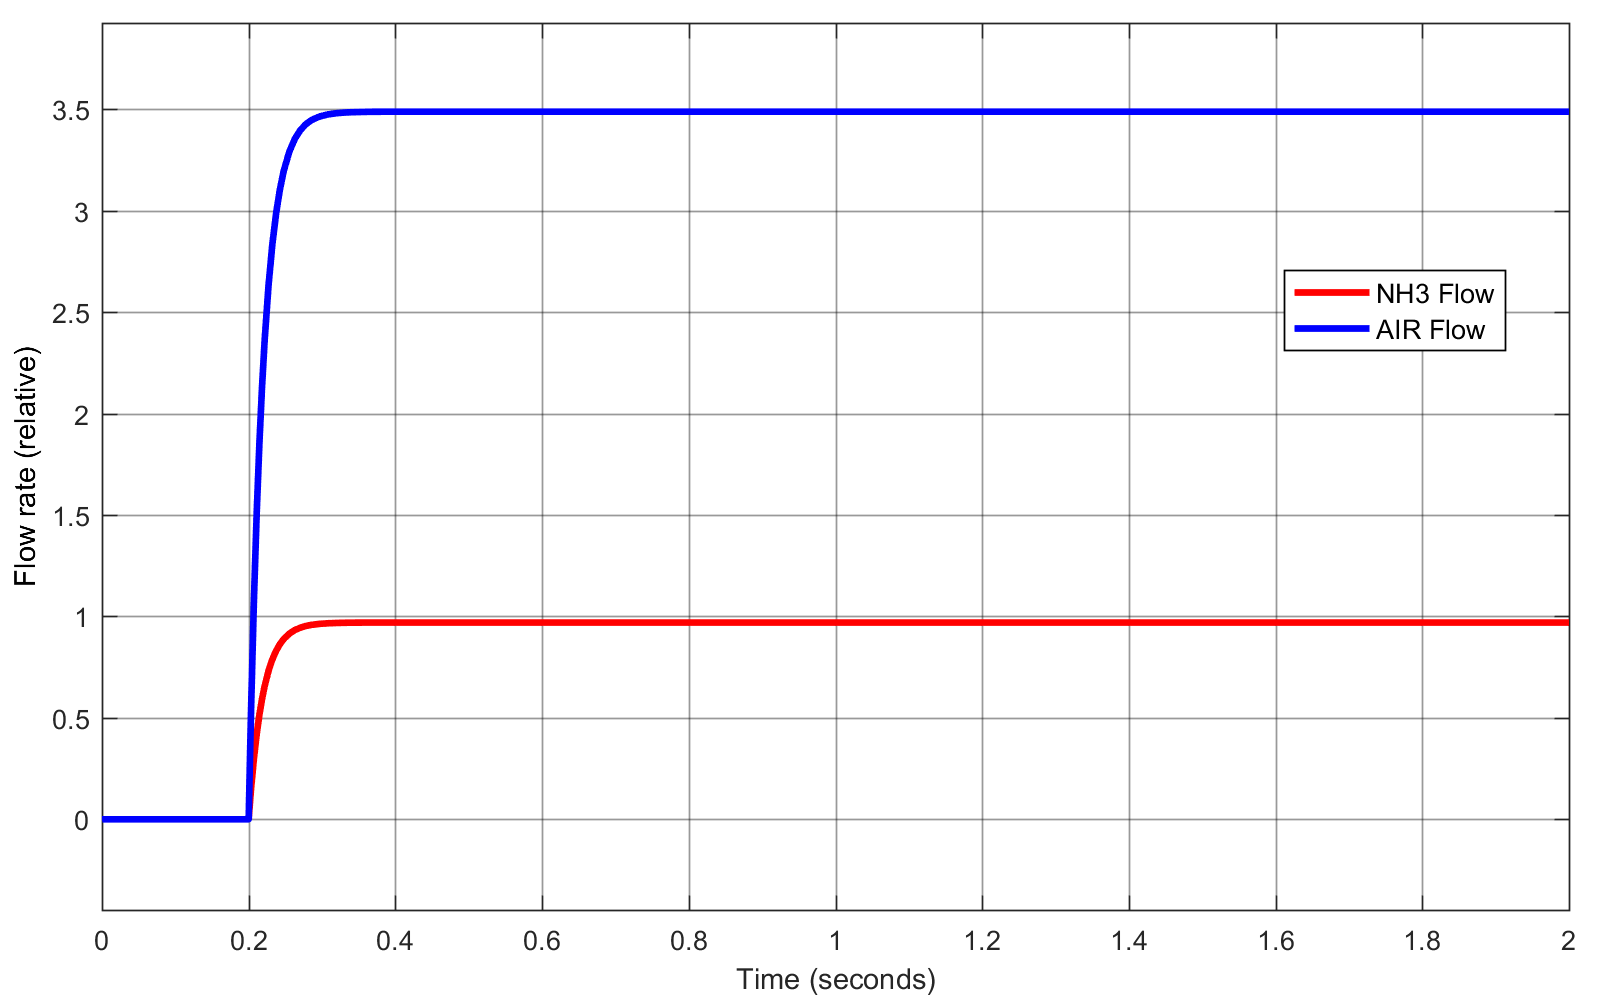
\includegraphics[scale=0.25]{controllerresponse.png}
    \caption{Caption}
    \label{fig:my_label}
\end{figure}

The block diagram of the controller is shown in Figure X, with the plant for each valve shown in Figure Y.

(DIAGRAM)
\begin{figure}[htb]
    \centering
    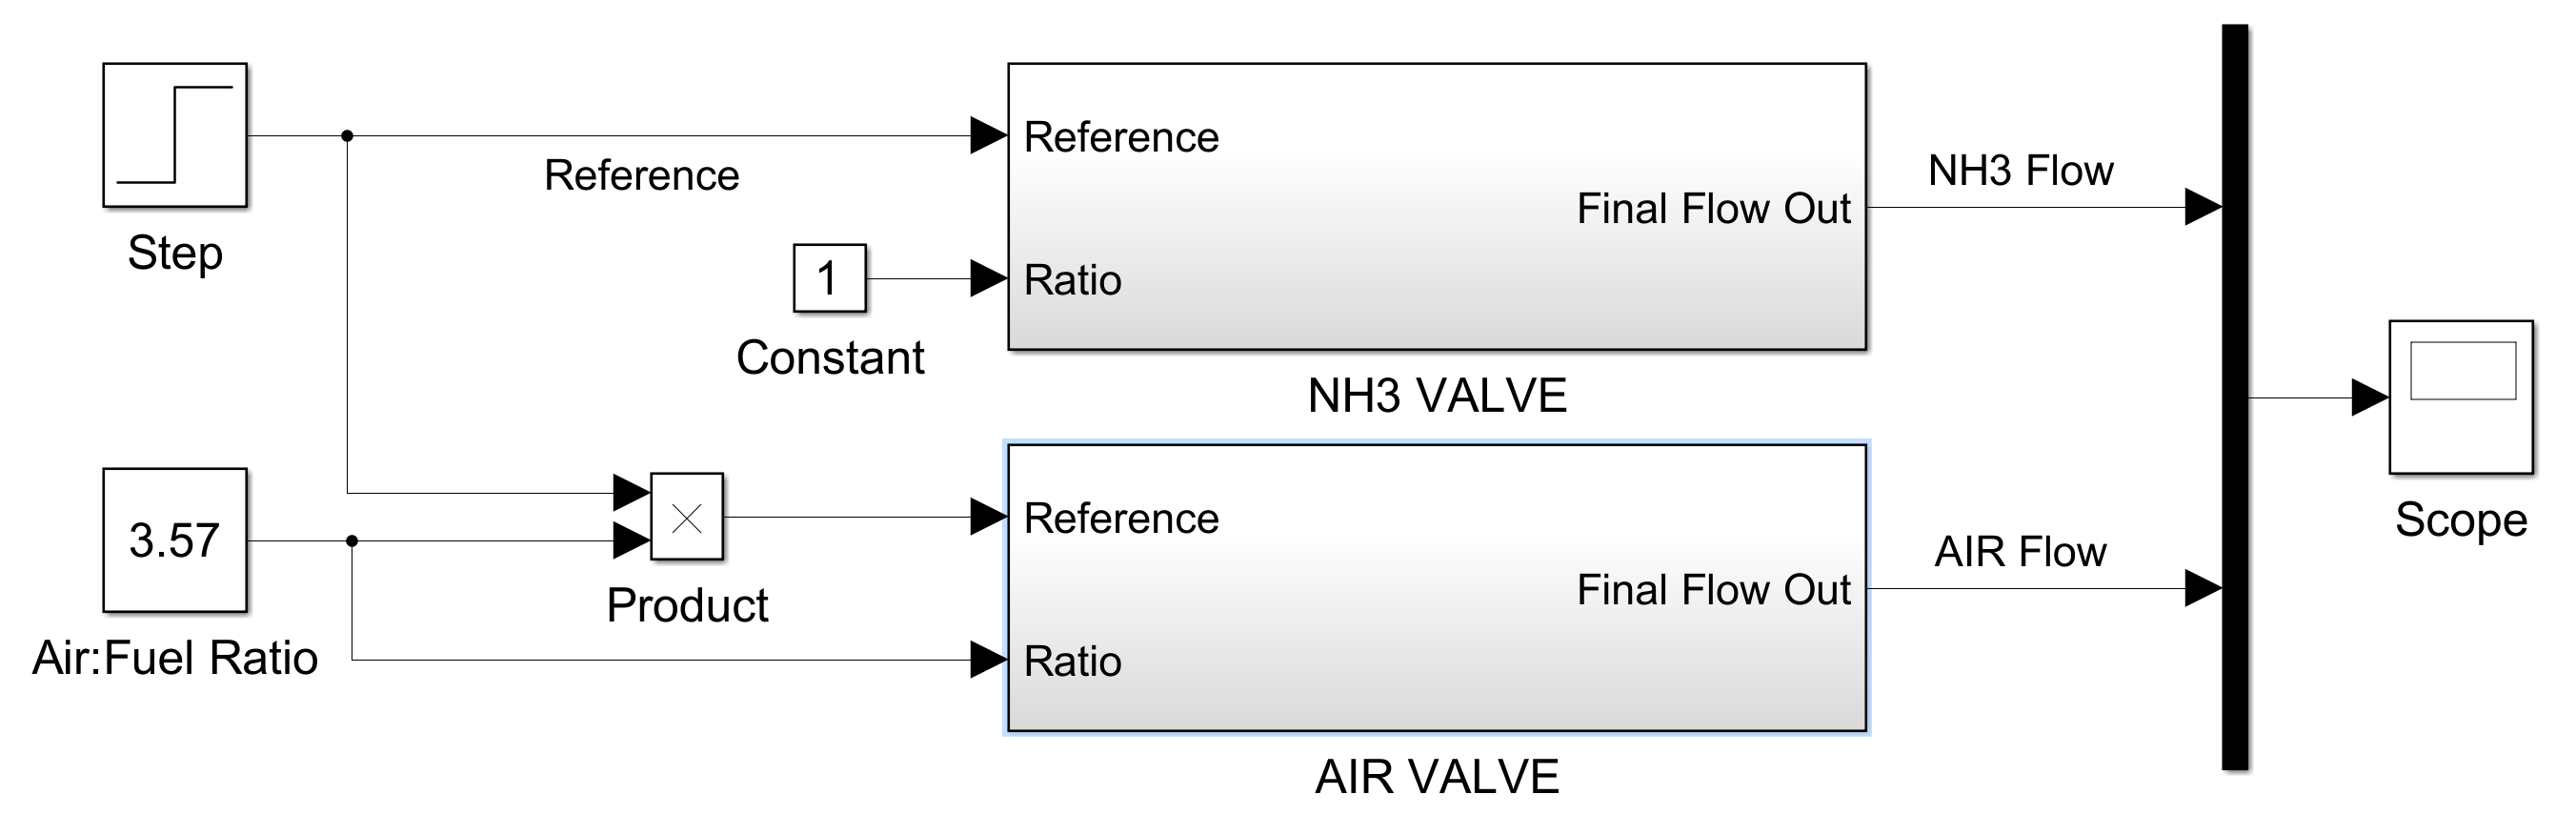
\includegraphics[scale=0.23]{controlleroverall.png}
    \caption{Caption}
    \label{fig:my_label}
\end{figure}

\begin{sidewaysfigure}[p]
    \centering
    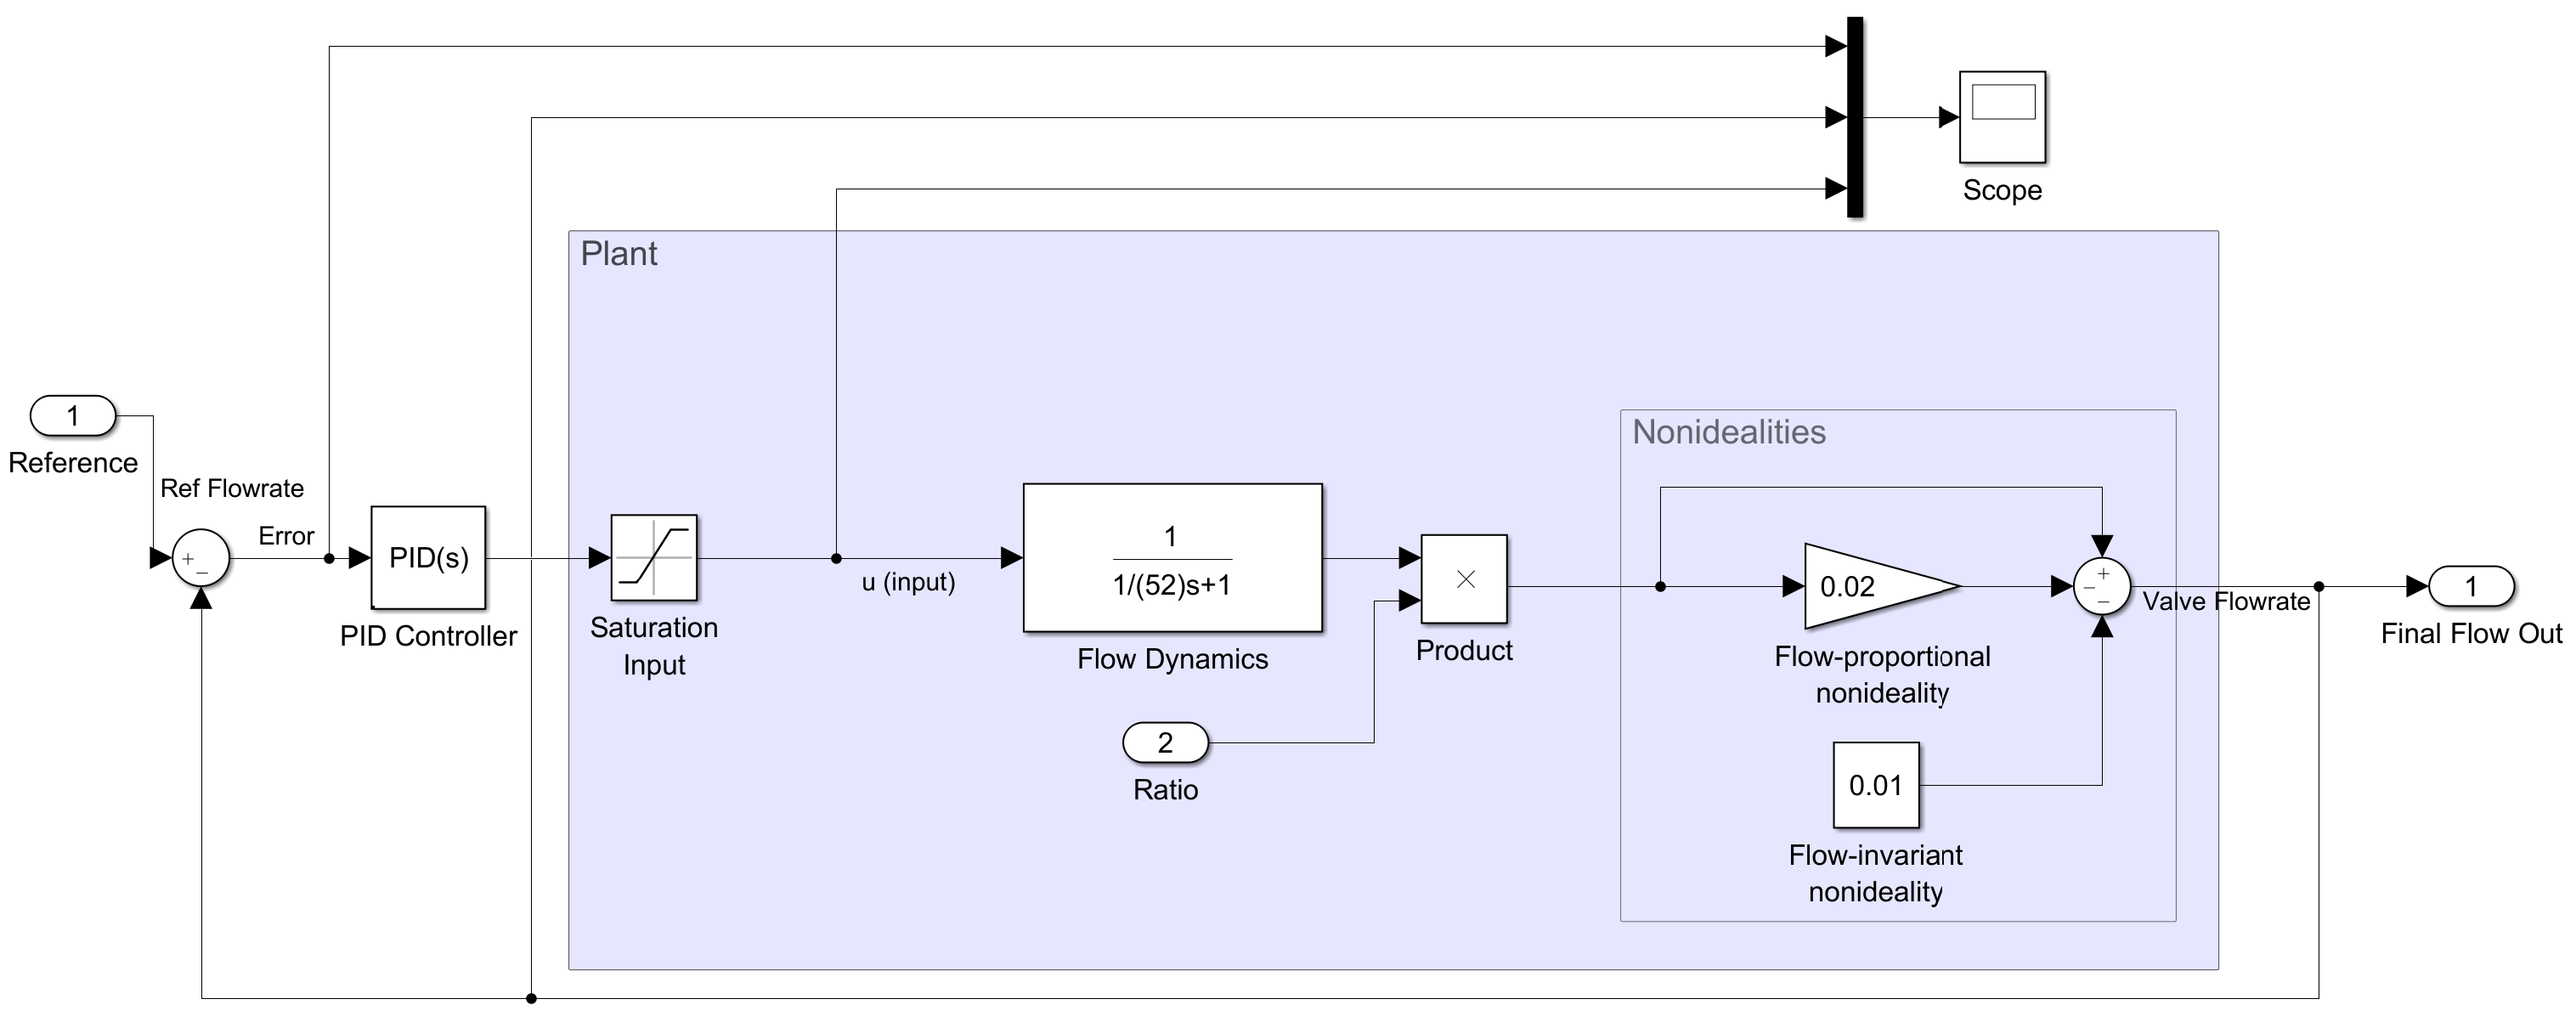
\includegraphics[scale=0.8]{valvecontroller.png}
    \caption{Caption}
    \label{fig:my_label}
\end{sidewaysfigure}


\subsection{System Overview}
Table 4 gives on overview of the SOFC-gas turbine system characteristics. The overall efficiency of the system is calculated by the useful power output divided by the total energy of the fuel input:
\begin{equation}
\eta_{overall}=  \frac{\text{Total power out}}{(〖LHV〗_{NH3}* \dot{m}_{NH_3})}				
\end{equation}
Where $LHV_{NH_3}$ is the ‘lower heating value’ of ammonia (found to be 18.6MJ/kg[25]), and $\dot{m}_{NH_3}$ is the total mass flow rate of ammonia into the SOFC.

TABLE
\begin{table}[h!]
\centering
\caption{My caption}
\label{my-label}
\begin{tabular}{|c|c|}
\hline
Number of cells per stack                 & 1150   \\ \hline
Maximum power output of single stack (MW) & 1.0    \\ \hline
Number of fuel cells stacks               & 150    \\ \hline
Notal net power from SOFC (MW)            & 150    \\ \hline
Total net power from turbine cycle (MW)   & 80     \\ \hline
Overall efficiency                        & 62.7\% \\ \hline
\end{tabular}
\end{table}

\subsection{Cost Analysis} 
The purchase cost per kW generated of the various components are shown in Table 5. The cost of the SOFC accounts for the cost of manufacture and testing, as well as accounting for various auxiliary systems such as the electronics, controls and sensory instruments, and assumes a sale price mark up of 50\%. The final value given in the report also includes the supply of fuel, air and water – these values have been removed from the total, giving \$6200 per kW[21]. The gas cycle components were found to be \$700 per kW generated[22]. The heat exchanger costs were calculated using[23]:
\begin{equation}
C_{HEX}=130\Big ( \frac{A}{0.093}\Big )	^{0.78} 					
\end{equation}
Where $C_{HEX}$ is the cost of the heat exchanger in USD, and $A$ is the area of the heat exchanger in square metres.

TABLE
\begin{table}[h!]
\centering
\caption{My caption}
\label{my-label}
\begin{tabular}{|c|c|c|}
\hline
\textbf{Component}      & \textbf{Cost per kW (USD)} & \textbf{Total Cost (millions of USD)} \\ \hline
Fuel Cells              & 1.0                        & 930                                   \\ \hline
Gas Cycles              & 150                        & 56                                    \\ \hline
\textbf{Heat Exchanger} & \textbf{Area (m2)}         & \textbf{Cost (millions of USD)}       \\ \hline
HEX 1                   & 710                        & 0.14                                  \\ \hline
HEX 2                   & 2185                       & 0.33                                  \\ \hline
HEX 3                   & 14255                      & 1.44                                  \\ \hline
\end{tabular}
\end{table}
The fuel cells have a life span of approximately 5.5 years, so will need to be replaced every 5 years[24]. The total costs, including operation, labour costs and maintenance costs, are dealt with in detail in section "!!!!!!!!!"

\subsection{Sustainability Analysis}
The integrated SOFC-gas turbine system is sustainable by design. The SOFC produces no particulate matter, or greenhouse gases[], and despite concerns about the production of nitrous oxides, these concerns have been shown to be unnecessary as the high operating temperature of the fuel cells mean the reaction is almost entirely complete[]. As such, NOx production is negligible, provided the SOFC system is run at the specified temperature. The fuel cells themselves are constructed from very common materials, so there is no danger of any material shortage in future. Unlike most fuel cells that run on hydrocarbons, the ammonia-fed fuel cell doesn’t coke[], giving it a much longer life span than usual. The gas turbines are fed entirely with atmospheric air, and heated using the exhaust from the fuel cells. The combination of the fuel cells with the gas turbines significantly increases the efficiency of the system – up to 60\% in this case - much more efficient than conventional power generation methods, which are typically around 40\% efficient[19].
\subsection{Safety and Risk Analysis}
A Hazard and Operability (HAZOP) analysis was performed on the plan for the SOFC system in order to identify any potential risks of danger to personnel, as well as damage to the system itself.

HAZOP TABLE
\begin{table}
\centering
\caption{My caption}
\label{my-label}
\renewcommand{\arraystretch}{1.5}
\begin{tabular}{|A|B|B|B|B|}
\hline
Guide Word & Deviation & Cause & \textbf{Consequence} & \textbf{Action} \\ \hline
\multirow{7}{*}{NO} & \multirow{2}{*}{Air flow} & Pipe Leakage & \multirow{2}{*}{No reaction, \\therefore no power output} & \multirow{2}{*}{Regular inspection of air flow equipment} \\ \cline{3-3}
 &  & Damage to air inlet &  &  \\ \cline{2-5} 
 & \multirow{3}{*}{Fuel Flow} & Pipe leakage & \multirow{3}{*}{\begin{tabular}[B]{@{}c@{}}No reaction, therefore no power output\\ Ammonia leakage can ignite, and is toxic to humans\end{tabular}} & Regular inspection of fuel flow equipment \\ \cline{3-3} \cline{5-5} 
 &  & Damage to fuel inlet &  & \multirow{2}{*}{Check the ammonia storage/production facilities} \\ \cline{3-3}
 &  & No ammonia in storage/being produced &  &  \\ \cline{2-5} 
 & Heat input to SOFC stacks & Faulty Heater & \begin{tabular}[B]{@{}c@{}}SOFC’s can’t be\\   operated when needed\end{tabular} & \begin{tabular}[B]{@{}c@{}}Regular inspection\\   of heater\end{tabular} \\ \cline{2-5} 
 & Electricity output & Faulty wiring & No power output & \begin{tabular}[B]{@{}c@{}}Regular\\   inspection\end{tabular} \\ \hline
\multirow{3}{*}{MORE} & Air flow & \multirow{3}{*}{Faulty controller, SOFC not operating as required} & \begin{tabular}[B]{@{}c@{}}Plant efficiency\\   decreases\end{tabular} & \multirow{3}{*}{\begin{tabular}[B]{@{}c@{}}Regular\\   inspection of controller,\\   Design system to\\   notify control staff\end{tabular}} \\ \cline{2-2} \cline{4-4}
 & Fuel flow &  & \begin{tabular}[B]{@{}c@{}}Fuel utilisation\\   decreases\end{tabular} &  \\ \cline{2-2} \cline{4-4}
 & Power output &  & \begin{tabular}[B]{@{}c@{}}Wasted power\\   production\end{tabular} &  \\ \hline
\multirow{2}{*}{LESS} & Air flow & \multirow{2}{*}{\begin{tabular}[B]{@{}c@{}}Faulty\\   controller, \\   SOFC not\\   operating as required\end{tabular}} & \multirow{2}{*}{\begin{tabular}[B]{@{}c@{}}Power output\\   reduced\end{tabular}} & \multirow{2}{*}{As above} \\ \cline{2-2}
 & Fuel flow &  &  &  \\ \hline
\multirow{3}{*}{AS WELL AS} & \begin{tabular}[B]{@{}c@{}}Air\\   contamination\end{tabular} & \begin{tabular}[B]{@{}c@{}}Surrounding air\\   in contaminated\end{tabular} & \begin{tabular}[B]{@{}c@{}}Cathode active\\   sites become blocked with impurities\end{tabular} & \begin{tabular}[B]{@{}c@{}}Install air\\   filters at air inlet\end{tabular} \\ \cline{2-5} 
 & \begin{tabular}[B]{@{}c@{}}Fuel\\   contamination\end{tabular} & \begin{tabular}[B]{@{}c@{}}Faults with\\   storage or production facilities\end{tabular} & \begin{tabular}[B]{@{}c@{}}Anode active\\   sites become blocked with impurities\end{tabular} & \begin{tabular}[B]{@{}c@{}}Install filters\\   where possible, install contaminant sensors, cease operation with contaminated\\   fuel\end{tabular} \\ \cline{2-5} 
 & NOx in exhaust & \begin{tabular}[B]{@{}c@{}}Low temperature\\   reaction\end{tabular} & \begin{tabular}[B]{@{}c@{}}Harmful gases\\   released\end{tabular} & \begin{tabular}[B]{@{}c@{}}Install NOx\\   sensors in exhaust, do not allow operation below specified temperature\end{tabular} \\ \hline
PART OF & \begin{tabular}[B]{@{}c@{}}No reaction,\\   despite correct fuel and air flow\end{tabular} & \begin{tabular}[B]{@{}c@{}}Electrodes and\\   electrolytes are not connected properly/damaged\end{tabular} & No power output & \begin{tabular}[B]{@{}c@{}}Regular\\   inspection of SOFC stacks\end{tabular} \\ \hline
REVERSE & NA & NA & NA & NA \\ \hline
OTHER THAN & \begin{tabular}[B]{@{}c@{}}Start up/Shut\\   down\end{tabular} & Maintenance & \begin{tabular}[B]{@{}c@{}}Large\\   temperature change causes damage to cells due to expansion/contraction\end{tabular} & \begin{tabular}[B]{@{}c@{}}Minimise need\\   for additional maintenance\end{tabular} \\ \hline
\end{tabular}
\end{table}

\subsection{Considerations}
Several improvements could be made to the analysis in this project, with the most significant improvements being made to the SOFC model. Firstly, the more accurate Dusty-Gas Model could have been used, instead of the Extended Stefan-Maxwell Model, as it takes into account the effect of diffusion and permeation mechanics on the concentration of the reacting species[3]. Due to implementation problems however, the simpler Extended-Stefan-Maxwell model was used instead.
Secondly, the original intent of the model was to investigate a variety of different SOFC configurations, using different materials for the electrodes and electrolyte, and investigating the differences in performance between oxygen conducting SOFCs and hydrogen conducting SOFCs. However, due to the lack of literature and data regarding SOFC testing, there was very little variety in the materials used in the SOFCs, and a meta-study[] showing over 15 different configurations showed that the vast majority of electrodes and electrolytes were made of YSZ, with very minor differences due to different mixture compositions with other metals. For many of these mixtures, values for fundamental properties affecting SOFC performance were not available, and so could not be implemented properly into the model.
Finally, the heat exchangers could be designed in much greater detail, looking at non-dimensional numbers such as the Reynold’s number and the Nusselt number, which are based on the fluid properties but also the dimensions of the heat exchanger. This would allow for accurate values for the heat transfer coefficients. Heat losses could also be considered, as well as heat exchanger insulation. However, these changes are not so significant as the costs involved with the heat exchangers are negligible in comparison with the fuel cells themselves, and particuarly in the grand scheme of the plant economics.

\subsection{References}
1. https://en.wikipedia.org/wiki/Solid_oxide_fuel_cell (as seen 2/2018)

2. “Design & Development of planar solid oxide fuel cell”, Adolfo (2013)

3. “Energy & Exergy analyses of direct ammonia solid oxide fuel cell integrated with gas turbine power cycle”, Ishak et al. (2012)

4. “Definition and sensitivity analysis of a finite volume SOFC model for a tubular cell geometry”, Campanari, Iora (2004)

5. “Thermodynamic analysis of ammonia-fed solid oxide fuel cells”, Ishak et al. (2011).

6. “A review of numerical modelling of solid oxide fuel cells”, Kakaç et al. (2006)

7. “Implementing thermal management modelling into SOFC system-level design”, Kattke & Braun, (2010)

8. “CEP Magazine, online source - https://www.aiche.org/resources/publications/cep/2016/july/special-section-energy-solid-oxide-fuel-cells-and-membranes” (last accessed 7/4/2018)

9. “Cathode materials based on perovskite-like transition metal oxides for intermediate temperature solid oxide fuel cells”, Istomin & Antipov (2013)

10. “High Temperature Solid Oxide Fuel Cells (Fundamentals, Design and Applications)”, Singhal, C.S. and Kendall, K. (2003)

11. “Heat capacity and thermodynamic properties of lanthanum(III) chromate(III)”, Sakai & Stolen (1994)

12. “Morphology and thermal conductivity of yttria-stabilized zirconia coatings”, Zhao et al. (2006)

13. Neutrium, engineering education website – https://neutrium.net/heat_transfer/radiative-heat-transfer-coefficient/ (last accessed 9/4/2018)

14. European Insulation Manufacturers Association - https://www.eurima.org/about-mineral-wool/basics-of-heat-transfer.html
15. Engineering Toolbox - https://www.engineeringtoolbox.com/insulation-temperatures-d_922.html (last accessed 9/4/2018)

16. Engineering Toolbox - https://www.engineeringtoolbox.com/melting-temperature-metals-d_860.html (last accessed 14/4/2018)

17. “Dynamic performance analysis of a fuel-control valve for use in airbreathing engine research”, Butterton & Zeller, NASA technical note (1969)

18. “Handout: Step-by-step for Heat Exchanger Design”, Shawabkeh (2015)

19. EIA website - https://www.eia.gov/tools/faqs/faq.php?id=107&t=3

20. “A Total Cost of Ownership Model for Solid Oxide Fuel Cells in Combined Heat and Power and Power Only Applications”, Scataglini (2015)

21. “Manufacturing cost analysis of 1 KW and 5 KW Solid Oxide Fuel Cell (SOFC) for auxiliary power applications”, Battelle Memorial Institute (2014)

22. “Study of equipment prices in the power sector”, Pauschert (2009)

23. “Thermoeconomic Modeling and Parametric Study of Hybrid Solid Oxide Fuel Cell – Gas Turbine – Steam Turbine Power Plants Ranging from 1.5 MWe to 10 MWe”, Arsalis (2009)

24. “Towards a Large SOFC power plant”, Rosenburg et. Al (2010)

25. Space Propulsion Group website: http://www.spg-corp.com/clean-energy-power-generation.html (last accessed 19/4/2018)


%HOW TO MATH:
%$\frac{1}{x}$
%$\phi_{subscript}$
%$\phi^{superscript}$

%\end{document}
